% Options for packages loaded elsewhere
\PassOptionsToPackage{unicode}{hyperref}
\PassOptionsToPackage{hyphens}{url}
\PassOptionsToPackage{dvipsnames,svgnames,x11names}{xcolor}
%
\documentclass[
  11pt,
]{article}

\usepackage{amsmath,amssymb}
\usepackage{iftex}
\ifPDFTeX
  \usepackage[T1]{fontenc}
  \usepackage[utf8]{inputenc}
  \usepackage{textcomp} % provide euro and other symbols
\else % if luatex or xetex
  \usepackage{unicode-math}
  \defaultfontfeatures{Scale=MatchLowercase}
  \defaultfontfeatures[\rmfamily]{Ligatures=TeX,Scale=1}
\fi
\usepackage{lmodern}
\ifPDFTeX\else  
    % xetex/luatex font selection
    \setmainfont[]{Times New Roman}
\fi
% Use upquote if available, for straight quotes in verbatim environments
\IfFileExists{upquote.sty}{\usepackage{upquote}}{}
\IfFileExists{microtype.sty}{% use microtype if available
  \usepackage[]{microtype}
  \UseMicrotypeSet[protrusion]{basicmath} % disable protrusion for tt fonts
}{}
\makeatletter
\@ifundefined{KOMAClassName}{% if non-KOMA class
  \IfFileExists{parskip.sty}{%
    \usepackage{parskip}
  }{% else
    \setlength{\parindent}{0pt}
    \setlength{\parskip}{6pt plus 2pt minus 1pt}}
}{% if KOMA class
  \KOMAoptions{parskip=half}}
\makeatother
\usepackage{xcolor}
\usepackage[margin=2.5cm]{geometry}
\setlength{\emergencystretch}{3em} % prevent overfull lines
\setcounter{secnumdepth}{5}
% Make \paragraph and \subparagraph free-standing
\makeatletter
\ifx\paragraph\undefined\else
  \let\oldparagraph\paragraph
  \renewcommand{\paragraph}{
    \@ifstar
      \xxxParagraphStar
      \xxxParagraphNoStar
  }
  \newcommand{\xxxParagraphStar}[1]{\oldparagraph*{#1}\mbox{}}
  \newcommand{\xxxParagraphNoStar}[1]{\oldparagraph{#1}\mbox{}}
\fi
\ifx\subparagraph\undefined\else
  \let\oldsubparagraph\subparagraph
  \renewcommand{\subparagraph}{
    \@ifstar
      \xxxSubParagraphStar
      \xxxSubParagraphNoStar
  }
  \newcommand{\xxxSubParagraphStar}[1]{\oldsubparagraph*{#1}\mbox{}}
  \newcommand{\xxxSubParagraphNoStar}[1]{\oldsubparagraph{#1}\mbox{}}
\fi
\makeatother

\usepackage{color}
\usepackage{fancyvrb}
\newcommand{\VerbBar}{|}
\newcommand{\VERB}{\Verb[commandchars=\\\{\}]}
\DefineVerbatimEnvironment{Highlighting}{Verbatim}{commandchars=\\\{\}}
% Add ',fontsize=\small' for more characters per line
\usepackage{framed}
\definecolor{shadecolor}{RGB}{241,243,245}
\newenvironment{Shaded}{\begin{snugshade}}{\end{snugshade}}
\newcommand{\AlertTok}[1]{\textcolor[rgb]{0.68,0.00,0.00}{#1}}
\newcommand{\AnnotationTok}[1]{\textcolor[rgb]{0.37,0.37,0.37}{#1}}
\newcommand{\AttributeTok}[1]{\textcolor[rgb]{0.40,0.45,0.13}{#1}}
\newcommand{\BaseNTok}[1]{\textcolor[rgb]{0.68,0.00,0.00}{#1}}
\newcommand{\BuiltInTok}[1]{\textcolor[rgb]{0.00,0.23,0.31}{#1}}
\newcommand{\CharTok}[1]{\textcolor[rgb]{0.13,0.47,0.30}{#1}}
\newcommand{\CommentTok}[1]{\textcolor[rgb]{0.37,0.37,0.37}{#1}}
\newcommand{\CommentVarTok}[1]{\textcolor[rgb]{0.37,0.37,0.37}{\textit{#1}}}
\newcommand{\ConstantTok}[1]{\textcolor[rgb]{0.56,0.35,0.01}{#1}}
\newcommand{\ControlFlowTok}[1]{\textcolor[rgb]{0.00,0.23,0.31}{\textbf{#1}}}
\newcommand{\DataTypeTok}[1]{\textcolor[rgb]{0.68,0.00,0.00}{#1}}
\newcommand{\DecValTok}[1]{\textcolor[rgb]{0.68,0.00,0.00}{#1}}
\newcommand{\DocumentationTok}[1]{\textcolor[rgb]{0.37,0.37,0.37}{\textit{#1}}}
\newcommand{\ErrorTok}[1]{\textcolor[rgb]{0.68,0.00,0.00}{#1}}
\newcommand{\ExtensionTok}[1]{\textcolor[rgb]{0.00,0.23,0.31}{#1}}
\newcommand{\FloatTok}[1]{\textcolor[rgb]{0.68,0.00,0.00}{#1}}
\newcommand{\FunctionTok}[1]{\textcolor[rgb]{0.28,0.35,0.67}{#1}}
\newcommand{\ImportTok}[1]{\textcolor[rgb]{0.00,0.46,0.62}{#1}}
\newcommand{\InformationTok}[1]{\textcolor[rgb]{0.37,0.37,0.37}{#1}}
\newcommand{\KeywordTok}[1]{\textcolor[rgb]{0.00,0.23,0.31}{\textbf{#1}}}
\newcommand{\NormalTok}[1]{\textcolor[rgb]{0.00,0.23,0.31}{#1}}
\newcommand{\OperatorTok}[1]{\textcolor[rgb]{0.37,0.37,0.37}{#1}}
\newcommand{\OtherTok}[1]{\textcolor[rgb]{0.00,0.23,0.31}{#1}}
\newcommand{\PreprocessorTok}[1]{\textcolor[rgb]{0.68,0.00,0.00}{#1}}
\newcommand{\RegionMarkerTok}[1]{\textcolor[rgb]{0.00,0.23,0.31}{#1}}
\newcommand{\SpecialCharTok}[1]{\textcolor[rgb]{0.37,0.37,0.37}{#1}}
\newcommand{\SpecialStringTok}[1]{\textcolor[rgb]{0.13,0.47,0.30}{#1}}
\newcommand{\StringTok}[1]{\textcolor[rgb]{0.13,0.47,0.30}{#1}}
\newcommand{\VariableTok}[1]{\textcolor[rgb]{0.07,0.07,0.07}{#1}}
\newcommand{\VerbatimStringTok}[1]{\textcolor[rgb]{0.13,0.47,0.30}{#1}}
\newcommand{\WarningTok}[1]{\textcolor[rgb]{0.37,0.37,0.37}{\textit{#1}}}

\providecommand{\tightlist}{%
  \setlength{\itemsep}{0pt}\setlength{\parskip}{0pt}}\usepackage{longtable,booktabs,array}
\usepackage{calc} % for calculating minipage widths
% Correct order of tables after \paragraph or \subparagraph
\usepackage{etoolbox}
\makeatletter
\patchcmd\longtable{\par}{\if@noskipsec\mbox{}\fi\par}{}{}
\makeatother
% Allow footnotes in longtable head/foot
\IfFileExists{footnotehyper.sty}{\usepackage{footnotehyper}}{\usepackage{footnote}}
\makesavenoteenv{longtable}
\usepackage{graphicx}
\makeatletter
\def\maxwidth{\ifdim\Gin@nat@width>\linewidth\linewidth\else\Gin@nat@width\fi}
\def\maxheight{\ifdim\Gin@nat@height>\textheight\textheight\else\Gin@nat@height\fi}
\makeatother
% Scale images if necessary, so that they will not overflow the page
% margins by default, and it is still possible to overwrite the defaults
% using explicit options in \includegraphics[width, height, ...]{}
\setkeys{Gin}{width=\maxwidth,height=\maxheight,keepaspectratio}
% Set default figure placement to htbp
\makeatletter
\def\fps@figure{htbp}
\makeatother

\usepackage{booktabs}
\usepackage{caption}
\usepackage{longtable}
\usepackage{colortbl}
\usepackage{array}
\usepackage{anyfontsize}
\usepackage{multirow}
\makeatletter
\@ifpackageloaded{caption}{}{\usepackage{caption}}
\AtBeginDocument{%
\ifdefined\contentsname
  \renewcommand*\contentsname{Table of contents}
\else
  \newcommand\contentsname{Table of contents}
\fi
\ifdefined\listfigurename
  \renewcommand*\listfigurename{List of Figures}
\else
  \newcommand\listfigurename{List of Figures}
\fi
\ifdefined\listtablename
  \renewcommand*\listtablename{List of Tables}
\else
  \newcommand\listtablename{List of Tables}
\fi
\ifdefined\figurename
  \renewcommand*\figurename{Figure}
\else
  \newcommand\figurename{Figure}
\fi
\ifdefined\tablename
  \renewcommand*\tablename{Table}
\else
  \newcommand\tablename{Table}
\fi
}
\@ifpackageloaded{float}{}{\usepackage{float}}
\floatstyle{ruled}
\@ifundefined{c@chapter}{\newfloat{codelisting}{h}{lop}}{\newfloat{codelisting}{h}{lop}[chapter]}
\floatname{codelisting}{Listing}
\newcommand*\listoflistings{\listof{codelisting}{List of Listings}}
\makeatother
\makeatletter
\makeatother
\makeatletter
\@ifpackageloaded{caption}{}{\usepackage{caption}}
\@ifpackageloaded{subcaption}{}{\usepackage{subcaption}}
\makeatother

\ifLuaTeX
  \usepackage{selnolig}  % disable illegal ligatures
\fi
\usepackage{bookmark}

\IfFileExists{xurl.sty}{\usepackage{xurl}}{} % add URL line breaks if available
\urlstyle{same} % disable monospaced font for URLs
\hypersetup{
  colorlinks=true,
  linkcolor={blue},
  filecolor={Maroon},
  citecolor={Blue},
  urlcolor={Blue},
  pdfcreator={LaTeX via pandoc}}


\author{}
\date{}

\begin{document}

\begin{titlepage}
    \noindent
    \begin{flushleft}
        \textbf{James Lewis} \\
    \end{flushleft}

    \vspace*{0.8cm}
    \centering

    \centering
    \vspace*{1.5cm}

    
\includegraphics[width=0.42\textwidth]{Uni-Exeter-logo-portrait-1.png}\par\vspace{1.2cm}

    {\scshape\Large University of Exeter \par}
    \vspace{1.2cm}

    {\Huge\bfseries Assessment \par}
    \vspace{0.6cm}

    {\large Module Code: MTHM505 – Data Science And Statistical Modelling In Space And Time\par}
    
    \vspace*{0.8cm}

    \small
    \noindent\rule{\textwidth}{0.4pt}
    \vspace{0.2cm}

    \textbf{Declaration of AI Assistance} \\
    I have used OpenAI’s ChatGPT tool in creating this report. \\

    AI-supported/AI-integrated use is permitted in this assessment. I acknowledge the following uses of GenAI tools in this assessment:

    \begin{itemize}\itemsep0pt \topsep0pt \parsep0pt
      \item Checking and debugging code
      \item Proofreading grammar and spelling
      \item Providing feedback on a draft
    \end{itemize}

    \vspace{-0.2cm}
    I declare that I have referenced use of GenAI outputs within my assessment in line with the University referencing guidelines.

\end{titlepage}

\renewcommand*\contentsname{Table of contents}
{
\hypersetup{linkcolor=}
\setcounter{tocdepth}{3}
\tableofcontents
}

\newpage

\section{Sea Surface Temperature
Modelling}\label{sea-surface-temperature-modelling}

\subsection{Part A: Cleaning and Spatial
Overview}\label{part-a-cleaning-and-spatial-overview}

\begin{figure}[H]

{\centering 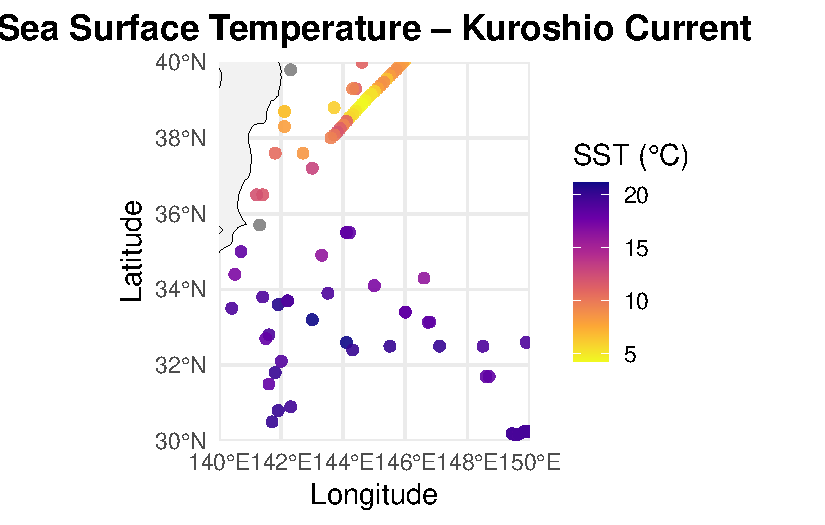
\includegraphics{project_files/figure-pdf/fig-scatterplot-1.pdf}

}

\caption{Figure 1: Spatial distribution of Sea Surface Temperature (SST)
observations collected on 1--2 January 1996 in the Kuroshio Current
region. Each point represents an individual measurement; colour denotes
temperature, with warmer SSTs concentrated in the north-east band.}

\end{figure}%

The dataset \texttt{kuroshio100.csv} contains 100 sea surface
temperature (SST) observations from January 1996, recorded along the
Kuroshio current system. Initial data inspection revealed three rows
with missing spatial coordinates (\texttt{lon} or \texttt{lat}), which
were removed to ensure compatibility with spatial modelling functions
such as \texttt{as.geodata()}.

This resulted in \textbf{97 complete observations}, covering a broad
range of longitudes and latitudes in the western Pacific Ocean. These
values were retained for further exploratory and model-based analysis.

Figure 1 confirms the dataset captures a wide latitudinal spread and a
broad SST range. Warmer values were observed to the south and east,
suggesting a clear spatial structure that will be investigated in
subsequent sections.

I should comment on that weird pattern of data!

\subsection{Part B: Spatial Data Partitioning for
Validation}\label{part-b-spatial-data-partitioning-for-validation}

To enable independent model validation, five spatial locations were
randomly withheld from the dataset. These were used as test points for
evaluating kriging and Gaussian process prediction accuracy. The
selection was made using a fixed seed for reproducibility:

\begin{Shaded}
\begin{Highlighting}[]
\FunctionTok{set.seed}\NormalTok{(}\DecValTok{444}\NormalTok{)  }\CommentTok{\# For reproducibility}

\CommentTok{\# Using the cleaned dataset to ensure we dont chose missing values.}
\CommentTok{\# 5 random points}
\NormalTok{test\_points }\OtherTok{\textless{}{-}}\NormalTok{ kuroshio100\_clean }\SpecialCharTok{\%\textgreater{}\%}
  \FunctionTok{sample\_n}\NormalTok{(}\DecValTok{5}\NormalTok{)}

\CommentTok{\# Display their information}
\NormalTok{test\_points }\SpecialCharTok{\%\textgreater{}\%}
  \FunctionTok{select}\NormalTok{(id, lon, lat, sst)}
\end{Highlighting}
\end{Shaded}

\begin{verbatim}
         id    lon   lat  sst
1      MQWU 142.10 38.70  6.5
2 49  16760 145.40 39.56  6.5
3     21573 149.56 30.15 19.3
4     LATI4 140.70 35.00 18.2
5     3FFJ4 142.10 38.30  8.0
\end{verbatim}

Now we create the training dataset

\begin{Shaded}
\begin{Highlighting}[]
\CommentTok{\# Create training dataset (excluding test points)}
\NormalTok{kuroshio\_train }\OtherTok{\textless{}{-}} \FunctionTok{anti\_join}\NormalTok{(kuroshio100, test\_points, }\AttributeTok{by =} \FunctionTok{c}\NormalTok{(}\StringTok{"id"}\NormalTok{, }\StringTok{"lon"}\NormalTok{, }\StringTok{"lat"}\NormalTok{, }\StringTok{"sst"}\NormalTok{))}

\CommentTok{\# Save for later prediction}
\NormalTok{test\_coords }\OtherTok{\textless{}{-}}\NormalTok{ test\_points }\SpecialCharTok{\%\textgreater{}\%} \FunctionTok{select}\NormalTok{(lon, lat)}
\NormalTok{test\_true\_sst }\OtherTok{\textless{}{-}}\NormalTok{ test\_points }\SpecialCharTok{\%\textgreater{}\%} \FunctionTok{select}\NormalTok{(sst)}
\end{Highlighting}
\end{Shaded}

This split produced:

\begin{itemize}
\item
  \textbf{Training set}: 92 spatial observations
\item
  \textbf{Test set}: 5 observations reserved for validation
\end{itemize}

These five test points are used consistently in Parts C--E to compare
model predictions and assess uncertainty quantification.

\subsection{Part C: Empirical Variogram and Spatial Correlation
Structure}\label{part-c-empirical-variogram-and-spatial-correlation-structure}

CHECK IS MAX DIST IS RIGHT, CHECK IF I NEED TO INCLUDE TREND IN
VARIOGRAM

USE WEEK 2 PRACTICAL.

Let sample variogram do itslef, I am overcolpicated bins etc

data(parana) par(mar=c(4,2,2,2)) plot(parana)

Refer to this for trend??\\

\begin{Shaded}
\begin{Highlighting}[]
\CommentTok{\# Convert training dataset into a geodata object}
\CommentTok{\# kuro\_geo\_train \textless{}{-} as.geodata(kuroshio\_train, coords.col = c("lon", "lat"), data.col = "sst")}

\CommentTok{\# Jitter duplicated coordinates very slightly}
\NormalTok{kuro\_geo\_train }\OtherTok{\textless{}{-}} \FunctionTok{jitterDupCoords}\NormalTok{(}
  \FunctionTok{as.geodata}\NormalTok{(kuroshio\_train, }\AttributeTok{coords.col =} \FunctionTok{c}\NormalTok{(}\StringTok{"lon"}\NormalTok{, }\StringTok{"lat"}\NormalTok{), }\AttributeTok{data.col =} \StringTok{"sst"}\NormalTok{),}
  \AttributeTok{max =} \FloatTok{1e{-}5}
\NormalTok{)}
\end{Highlighting}
\end{Shaded}

\begin{verbatim}
as.geodata: 19 replicated data locations found. 
 Consider using jitterDupCoords() for jittering replicated locations. 
WARNING: there are data at coincident or very closed locations, some of the geoR's functions may not work.
 Use function dup.coords() to locate duplicated coordinates.
 Consider using jitterDupCoords() for jittering replicated locations 
\end{verbatim}

\texttt{max\ =\ 1e-5} means the jitter is on the order of 0.00001
degrees --- negligible in geographic terms. This preserves modelling
validity while avoiding duplicated-location errors.

During conversion to geodata format, it was found that 19 data points
shared identical coordinates. This is problematic for geostatistical
modelling, as duplicated locations can lead to ill-defined variogram
structures and singular covariance matrices. To address this, we applied
a minimal spatial jitter using \texttt{jitterDupCoords()}, introducing
negligible noise to break coordinate ties while preserving the
underlying spatial pattern.

\subsubsection{Empirical Variogram
Estimation}\label{empirical-variogram-estimation}

\begin{Shaded}
\begin{Highlighting}[]
\CommentTok{\# Empirical variogram with binning}
\CommentTok{\# Full range}
\NormalTok{emp\_variog\_full }\OtherTok{\textless{}{-}} \FunctionTok{variog}\NormalTok{(kuro\_geo\_train, }\AttributeTok{option =} \StringTok{"bin"}\NormalTok{, }\AttributeTok{max.dist =} \FloatTok{2.5}\NormalTok{, }\AttributeTok{uvec =} \FunctionTok{seq}\NormalTok{(}\DecValTok{0}\NormalTok{, }\FloatTok{2.5}\NormalTok{, }\AttributeTok{length.out =} \DecValTok{20}\NormalTok{))}
\end{Highlighting}
\end{Shaded}

\begin{verbatim}
variog: computing omnidirectional variogram
\end{verbatim}

\begin{Shaded}
\begin{Highlighting}[]
\CommentTok{\# Mid{-}range (preferred candidate for fitting)}
\NormalTok{emp\_variog\_2 }\OtherTok{\textless{}{-}} \FunctionTok{variog}\NormalTok{(kuro\_geo\_train, }\AttributeTok{option =} \StringTok{"bin"}\NormalTok{, }\AttributeTok{max.dist =} \FloatTok{2.0}\NormalTok{, }\AttributeTok{uvec =} \FunctionTok{seq}\NormalTok{(}\DecValTok{0}\NormalTok{, }\FloatTok{2.0}\NormalTok{, }\AttributeTok{length.out =} \DecValTok{20}\NormalTok{))}
\end{Highlighting}
\end{Shaded}

\begin{verbatim}
variog: computing omnidirectional variogram
\end{verbatim}

\begin{Shaded}
\begin{Highlighting}[]
\CommentTok{\# Cleanest for model fitting}
\NormalTok{emp\_variog\_1}\FloatTok{.8} \OtherTok{\textless{}{-}} \FunctionTok{variog}\NormalTok{(kuro\_geo\_train, }\AttributeTok{option =} \StringTok{"bin"}\NormalTok{, }\AttributeTok{max.dist =} \FloatTok{1.8}\NormalTok{, }\AttributeTok{uvec =} \FunctionTok{seq}\NormalTok{(}\DecValTok{0}\NormalTok{, }\FloatTok{1.8}\NormalTok{, }\AttributeTok{length.out =} \DecValTok{18}\NormalTok{))}
\end{Highlighting}
\end{Shaded}

\begin{verbatim}
variog: computing omnidirectional variogram
\end{verbatim}

To assess the spatial dependence in SST, the semi-variance is computed
as:

\[
\gamma(h) = \frac{1}{2N(h)} \sum_{\substack{i,j: \\ \|s_i - s_j\| \approx h}} \left( z(s_i) - z(s_j) \right)^2
\]

where:

\begin{itemize}
\item
  \(N(h)\) is the number of location pairs separated by distance hhh,
\item
  \$s\_i\$\hspace{0pt} and \$s\_j\$\hspace{0pt} are spatial coordinates
  of observations,
\item
  \(z\)\((s_i)\) is the SST value at location \(s_i\)\hspace{0pt}.
\end{itemize}

The semi-variance \(\gamma(h)\) increases with distance \(h\) if spatial
correlation is present.

\begin{figure}[H]

{\centering 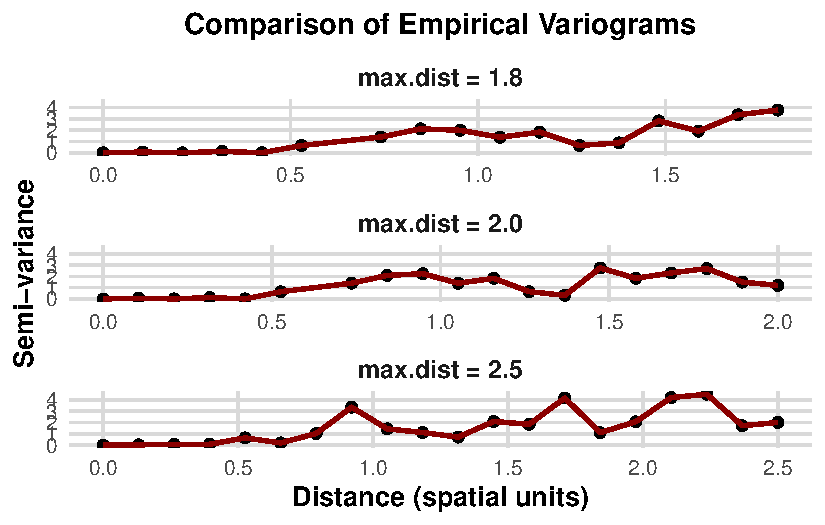
\includegraphics{project_files/figure-pdf/fig-variogcompare-1.pdf}

}

\caption{Figure 2: Empirical variograms computed using three different
maximum distance thresholds. The max.dist = 1.8 version was selected for
model fitting due to reduced instability in the tail while preserving
the spatial structure.}

\end{figure}%

Empirical variograms were computed using the \texttt{variog()} function
in \texttt{geoR}, with binned distance lags defined via \texttt{uvec}.
Three distance thresholds were tested --- \texttt{max.dist\ =\ 2.5},
\texttt{2.0}, and \texttt{1.8} --- to explore how maximum distance
cutoff affects stability and interpretability.

\paragraph{Evaluation of Distance
Cutoffs}\label{evaluation-of-distance-cutoffs}

Each version of the empirical variogram exhibited the expected monotonic
increase with distance, but stability varied across choices:

\begin{itemize}
\item
  The \texttt{max.dist\ =\ 2.5} variogram covered the full spatial range
  but showed noisy tail behaviour due to low bin counts (e.g.~2--7
  observations).
\item
  The \texttt{max.dist\ =\ 2.0} improved stability but retained some
  variance at large distances.
\item
  The \texttt{max.dist\ =\ 1.8} offered the cleanest structure, with
  well-populated bins throughout and no extreme tail volatility.
\end{itemize}

Bin counts were monitored using \texttt{emp\_variog\$n}, and those for
the selected \texttt{max.dist\ =\ 1.8} were generally robust (e.g.,
\textgreater15 in most bins).

\paragraph{Nugget Effect
Justification}\label{nugget-effect-justification}

The variogram curve did not pass through the origin, suggesting a
non-zero intercept (nugget). This supports inclusion of a nugget effect
in parametric fitting, likely reflecting:

\begin{itemize}
\item
  Instrument noise
\item
  Sub-grid-scale oceanic variation
\end{itemize}

\paragraph{Final Selection}\label{final-selection}

The \texttt{max.dist\ =\ 1.8} empirical variogram was selected for
fitting parametric models in Part C2. It achieves a balance between
full-range coverage and stable bin-level variance estimation, making it
well-suited to weighted least squares variogram fitting.

\subsubsection{Fitting Parametric Variogram
Models}\label{fitting-parametric-variogram-models}

\begin{Shaded}
\begin{Highlighting}[]
\CommentTok{\#  Fit Parametric Variogram Models}
\CommentTok{\# Exponential model}
\NormalTok{fit\_exp }\OtherTok{\textless{}{-}} \FunctionTok{variofit}\NormalTok{(}
\NormalTok{  emp\_variog\_1}\FloatTok{.8}\NormalTok{,}
  \AttributeTok{cov.model =} \StringTok{"exponential"}\NormalTok{,}
  \AttributeTok{ini.cov.pars =} \FunctionTok{c}\NormalTok{(}\DecValTok{1}\NormalTok{, }\DecValTok{1}\NormalTok{),}
  \AttributeTok{nugget =} \FloatTok{0.1}\NormalTok{,}
  \AttributeTok{weights =} \StringTok{"equal"}
\NormalTok{)}
\end{Highlighting}
\end{Shaded}

\begin{verbatim}
variofit: covariance model used is exponential 
variofit: weights used: equal 
variofit: minimisation function used: optim 
\end{verbatim}

\begin{Shaded}
\begin{Highlighting}[]
\CommentTok{\# Gaussian model}
\NormalTok{fit\_gau }\OtherTok{\textless{}{-}} \FunctionTok{variofit}\NormalTok{(}
\NormalTok{  emp\_variog\_1}\FloatTok{.8}\NormalTok{,}
  \AttributeTok{cov.model =} \StringTok{"gaussian"}\NormalTok{,}
  \AttributeTok{ini.cov.pars =} \FunctionTok{c}\NormalTok{(}\DecValTok{1}\NormalTok{, }\DecValTok{1}\NormalTok{),}
  \AttributeTok{nugget =} \FloatTok{0.1}\NormalTok{,}
  \AttributeTok{weights =} \StringTok{"equal"}
\NormalTok{)}
\end{Highlighting}
\end{Shaded}

\begin{verbatim}
variofit: covariance model used is gaussian 
variofit: weights used: equal 
variofit: minimisation function used: optim 
\end{verbatim}

\begin{Shaded}
\begin{Highlighting}[]
\CommentTok{\# Adjusted first Matérn model as: sum of the nugget and partial sill initial values was too small. Two new improved models below:}

\CommentTok{\# Matérn model (kappa = 1.5)}
\NormalTok{fit\_mat1 }\OtherTok{\textless{}{-}} \FunctionTok{variofit}\NormalTok{(}
\NormalTok{  emp\_variog\_1}\FloatTok{.8}\NormalTok{,}
  \AttributeTok{cov.model =} \StringTok{"matern"}\NormalTok{,}
  \AttributeTok{kappa =} \FloatTok{1.5}\NormalTok{,}
  \AttributeTok{ini.cov.pars =} \FunctionTok{c}\NormalTok{(}\DecValTok{2}\NormalTok{, }\DecValTok{1}\NormalTok{),   }\CommentTok{\# partial sill = 2, range = 1}
  \AttributeTok{nugget =} \FloatTok{0.5}\NormalTok{,             }\CommentTok{\# starting nugget guess}
  \AttributeTok{weights =} \StringTok{"equal"}
\NormalTok{)}
\end{Highlighting}
\end{Shaded}

\begin{verbatim}
variofit: covariance model used is matern 
variofit: weights used: equal 
variofit: minimisation function used: optim 
\end{verbatim}

\begin{Shaded}
\begin{Highlighting}[]
\NormalTok{fit\_mat2 }\OtherTok{\textless{}{-}} \FunctionTok{variofit}\NormalTok{(}
\NormalTok{  emp\_variog\_1}\FloatTok{.8}\NormalTok{,}
  \AttributeTok{cov.model =} \StringTok{"matern"}\NormalTok{,}
  \AttributeTok{kappa =} \FloatTok{1.5}\NormalTok{,}
  \AttributeTok{ini.cov.pars =} \FunctionTok{c}\NormalTok{(}\FloatTok{1.5}\NormalTok{, }\FloatTok{0.8}\NormalTok{),}
  \AttributeTok{nugget =} \FloatTok{0.3}\NormalTok{,}
  \AttributeTok{weights =} \StringTok{"equal"}
\NormalTok{)}
\end{Highlighting}
\end{Shaded}

\begin{verbatim}
variofit: covariance model used is matern 
variofit: weights used: equal 
variofit: minimisation function used: optim 
\end{verbatim}

Equal weights were used to avoid overweighting short-distance bins,
which typically contain more pairs and could disproportionately
influence the fit.

\begin{figure}[H]

{\centering 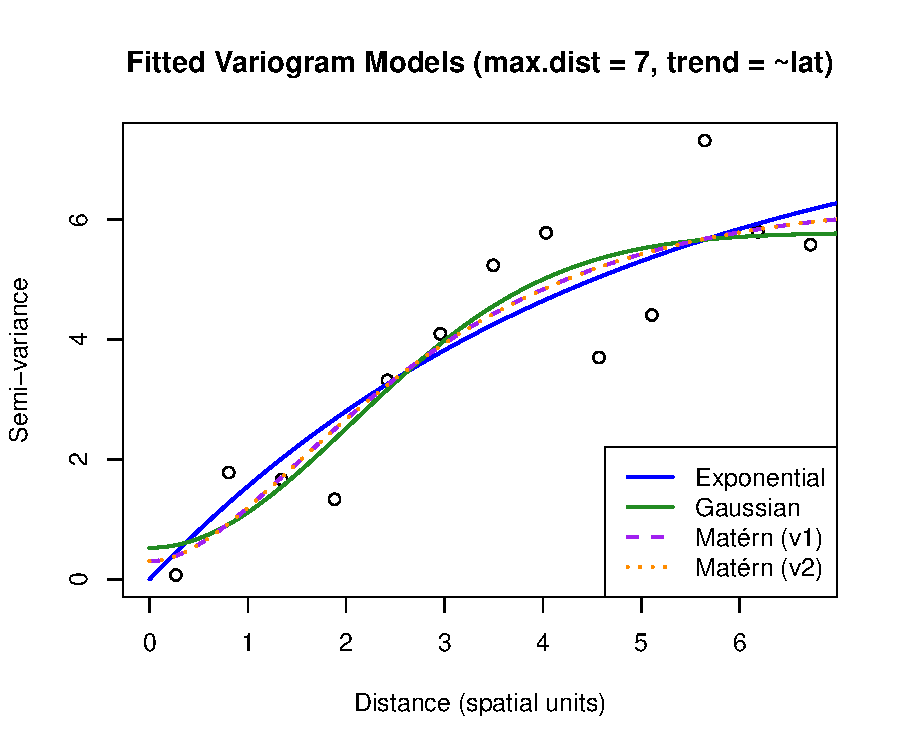
\includegraphics{project_files/figure-pdf/fig-variogfit-1.pdf}

}

\caption{Parametric variogram models (Exponential, Gaussian, Matérn)
fitted to the empirical variogram with max.dist = 1.8. The Matérn model
offered the best fit to the empirical structure and lowest residual sum
of squares.}

\end{figure}%

\begin{verbatim}
[1] 7.123255
\end{verbatim}

\begin{verbatim}
[1] 6.828983
\end{verbatim}

\begin{verbatim}
[1] 6.796541
\end{verbatim}

Parametric variogram models were fitted to the empirical variogram with
\texttt{max.dist\ =\ 1.8} using the \texttt{variofit()} function. Three
covariance functions were tested:

\begin{itemize}
\item
  \textbf{Exponential}: assumes rough sample paths and rapid correlation
  decay
\item
  \textbf{Gaussian}: assumes smooth sample paths with strong local
  correlation
\item
  \textbf{Matérn}: provides a flexible family; here set with
  κ=1.5\kappa = 1.5κ=1.5 for moderate smoothness
\end{itemize}

All models assumed:

\begin{itemize}
\item
  A \textbf{constant mean} function (i.e.~no trend component)
\item
  \textbf{Isotropy}, meaning spatial correlation depends only on
  Euclidean distance
\item
  \textbf{Second-order stationarity}
\item
  A \textbf{non-zero nugget}, motivated by the empirical variogram
\end{itemize}

Each model was fitted using weighted least squares. Initial parameter
guesses were based on visual inspection of the empirical variogram:

\subsubsection{\texorpdfstring{\textbf{Model Parameters and
Interpretation}}{Model Parameters and Interpretation}}\label{model-parameters-and-interpretation}

\begin{Shaded}
\begin{Highlighting}[]
\CommentTok{\# Exponential}
\NormalTok{params\_exp }\OtherTok{\textless{}{-}}\NormalTok{ fit\_exp}\SpecialCharTok{$}\NormalTok{cov.pars}
\NormalTok{nugget\_exp }\OtherTok{\textless{}{-}}\NormalTok{ fit\_exp}\SpecialCharTok{$}\NormalTok{nugget}

\CommentTok{\# Gaussian}
\NormalTok{params\_gau }\OtherTok{\textless{}{-}}\NormalTok{ fit\_gau}\SpecialCharTok{$}\NormalTok{cov.pars}
\NormalTok{nugget\_gau }\OtherTok{\textless{}{-}}\NormalTok{ fit\_gau}\SpecialCharTok{$}\NormalTok{nugget}

\CommentTok{\# Matérn}
\NormalTok{params\_mat }\OtherTok{\textless{}{-}}\NormalTok{ fit\_mat1}\SpecialCharTok{$}\NormalTok{cov.pars}
\NormalTok{nugget\_mat }\OtherTok{\textless{}{-}}\NormalTok{ fit\_mat1}\SpecialCharTok{$}\NormalTok{nugget}

\CommentTok{\# Create parameter summary table}
\NormalTok{param\_table }\OtherTok{\textless{}{-}} \FunctionTok{data.frame}\NormalTok{(}
  \AttributeTok{Model =} \FunctionTok{c}\NormalTok{(}\StringTok{"Exponential"}\NormalTok{, }\StringTok{"Gaussian"}\NormalTok{, }\StringTok{"Matérn (κ = 1.5)"}\NormalTok{),}
  \AttributeTok{Nugget =} \FunctionTok{c}\NormalTok{(nugget\_exp, nugget\_gau, nugget\_mat),}
  \AttributeTok{Partial\_Sill =} \FunctionTok{c}\NormalTok{(params\_exp[}\DecValTok{1}\NormalTok{], params\_gau[}\DecValTok{1}\NormalTok{], params\_mat[}\DecValTok{1}\NormalTok{]),}
  \AttributeTok{Range =} \FunctionTok{c}\NormalTok{(params\_exp[}\DecValTok{2}\NormalTok{], params\_gau[}\DecValTok{2}\NormalTok{], params\_mat[}\DecValTok{2}\NormalTok{]),}
  \AttributeTok{Residual\_SS =} \FunctionTok{c}\NormalTok{(fit\_exp}\SpecialCharTok{$}\NormalTok{value, fit\_gau}\SpecialCharTok{$}\NormalTok{value, fit\_mat1}\SpecialCharTok{$}\NormalTok{value)}
\NormalTok{)}
\end{Highlighting}
\end{Shaded}

\begin{longtable}[]{@{}
  >{\raggedright\arraybackslash}p{(\columnwidth - 8\tabcolsep) * \real{0.2432}}
  >{\raggedright\arraybackslash}p{(\columnwidth - 8\tabcolsep) * \real{0.1757}}
  >{\raggedright\arraybackslash}p{(\columnwidth - 8\tabcolsep) * \real{0.2568}}
  >{\raggedright\arraybackslash}p{(\columnwidth - 8\tabcolsep) * \real{0.1486}}
  >{\raggedright\arraybackslash}p{(\columnwidth - 8\tabcolsep) * \real{0.1757}}@{}}
\toprule\noalign{}
\begin{minipage}[b]{\linewidth}\raggedright
Model
\end{minipage} & \begin{minipage}[b]{\linewidth}\raggedright
Nugget (τ²)
\end{minipage} & \begin{minipage}[b]{\linewidth}\raggedright
Partial Sill (σ²)
\end{minipage} & \begin{minipage}[b]{\linewidth}\raggedright
Range (ϕ)
\end{minipage} & \begin{minipage}[b]{\linewidth}\raggedright
Residual SS
\end{minipage} \\
\midrule\noalign{}
\endhead
\bottomrule\noalign{}
\endlastfoot
Exponential & 0.000 & 4,208,359 & 2,718,693 & 7.12 \\
Gaussian & 0.255 & 282.69 & 17.22 & 6.83 \\
Matérn (κ = 1.5) & 0.180 & 26.68 & 3.13 & 6.80 \\
\end{longtable}

\textbf{Parametric Variogram Fitting and Selection}

Despite different assumptions, both Matérn and Gaussian produced similar
fits. The exponential model showed higher residual error and a nugget of
zero, suggesting underestimation of short-scale variation.

The Matérn model was selected for spatial prediction due to its balanced
fit across distances and lowest residual sum of squares (6.80). Its
parameters suggest a moderate range of spatial correlation (ϕ ≈ 3.13)
and a nugget variance of 0.18, indicating non-negligible unexplained
microscale variation. This model was used in the kriging stage.

\textbf{Spatial Prediction and Model Validation}

\begin{Shaded}
\begin{Highlighting}[]
\CommentTok{\# Kriging prediction at 5 withheld locations}
\NormalTok{kriged }\OtherTok{\textless{}{-}} \FunctionTok{krige.conv}\NormalTok{(}
  \AttributeTok{geodata =}\NormalTok{ kuro\_geo\_train,}
  \AttributeTok{locations =}\NormalTok{ test\_coords,}
  \AttributeTok{krige =} \FunctionTok{krige.control}\NormalTok{(}
    \AttributeTok{cov.model =} \StringTok{"matern"}\NormalTok{,}
    \AttributeTok{cov.pars =}\NormalTok{ fit\_mat1}\SpecialCharTok{$}\NormalTok{cov.pars,}
    \AttributeTok{nugget =}\NormalTok{ fit\_mat1}\SpecialCharTok{$}\NormalTok{nugget,}
    \AttributeTok{kappa =} \FloatTok{1.5}
\NormalTok{  )}
\NormalTok{)}
\end{Highlighting}
\end{Shaded}

\begin{verbatim}
krige.conv: model with constant mean
krige.conv: Kriging performed using global neighbourhood 
\end{verbatim}

\begin{Shaded}
\begin{Highlighting}[]
\CommentTok{\# Add predicted values and residuals}
\NormalTok{test\_results }\OtherTok{\textless{}{-}}\NormalTok{ test\_coords }\SpecialCharTok{\%\textgreater{}\%}
  \FunctionTok{mutate}\NormalTok{(}
    \AttributeTok{observed\_sst =}\NormalTok{ test\_true\_sst}\SpecialCharTok{$}\NormalTok{sst,}
    \AttributeTok{predicted\_sst =}\NormalTok{ kriged}\SpecialCharTok{$}\NormalTok{predict,}
    \AttributeTok{kriging\_var =}\NormalTok{ kriged}\SpecialCharTok{$}\NormalTok{krige.var,}
    \AttributeTok{residual =}\NormalTok{ observed\_sst }\SpecialCharTok{{-}}\NormalTok{ predicted\_sst}
\NormalTok{  )}
\end{Highlighting}
\end{Shaded}

Ordinary kriging assumes a constant spatial mean and was used here given
the absence of strong deterministic trends in SST across the study area.

\begin{figure}[H]

{\centering 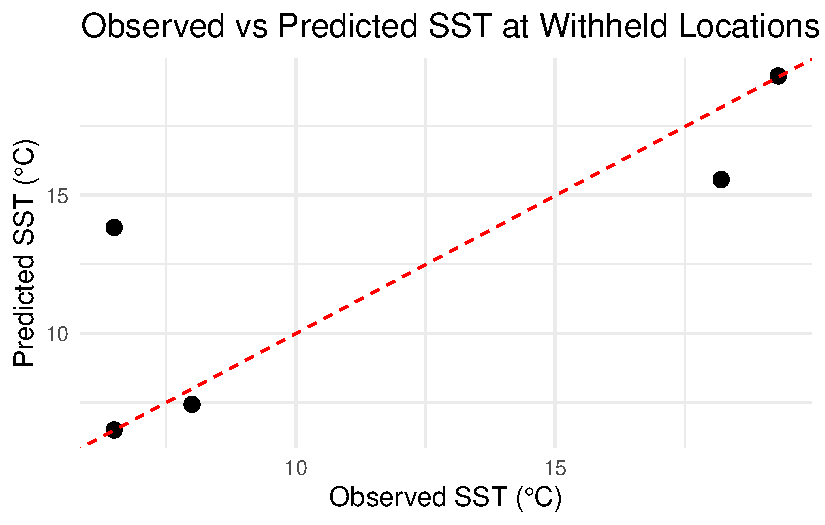
\includegraphics{project_files/figure-pdf/fig-krigscatter-1.pdf}

}

\caption{Observed vs predicted sea surface temperature (SST) at five
withheld locations using ordinary kriging with the fitted Matérn model.
Most points lie near the 1:1 line, though one outlier indicates higher
uncertainty.}

\end{figure}%

\begin{Shaded}
\begin{Highlighting}[]
\CommentTok{\# Perform LOOCV}
\NormalTok{xv.kriging }\OtherTok{\textless{}{-}} \FunctionTok{xvalid}\NormalTok{(kuro\_geo\_train, }\AttributeTok{model =}\NormalTok{ fit\_mat1)}
\end{Highlighting}
\end{Shaded}

\begin{verbatim}
xvalid: number of data locations       = 65
xvalid: number of validation locations = 65
xvalid: performing cross-validation at location ... 1, 2, 3, 4, 5, 6, 7, 8, 9, 10, 11, 12, 13, 14, 15, 16, 17, 18, 19, 20, 21, 22, 23, 24, 25, 26, 27, 28, 29, 30, 31, 32, 33, 34, 35, 36, 37, 38, 39, 40, 41, 42, 43, 44, 45, 46, 47, 48, 49, 50, 51, 52, 53, 54, 55, 56, 57, 58, 59, 60, 61, 62, 63, 64, 65, 
xvalid: end of cross-validation
\end{verbatim}

\begin{Shaded}
\begin{Highlighting}[]
\CommentTok{\# Plot residuals}
\FunctionTok{par}\NormalTok{(}\AttributeTok{mfrow =} \FunctionTok{c}\NormalTok{(}\DecValTok{3}\NormalTok{, }\DecValTok{2}\NormalTok{), }\AttributeTok{mar =} \FunctionTok{c}\NormalTok{(}\DecValTok{4}\NormalTok{, }\DecValTok{2}\NormalTok{, }\DecValTok{2}\NormalTok{, }\DecValTok{2}\NormalTok{))}
\FunctionTok{plot}\NormalTok{(xv.kriging, }\AttributeTok{error =} \ConstantTok{TRUE}\NormalTok{, }\AttributeTok{std.error =} \ConstantTok{FALSE}\NormalTok{, }\AttributeTok{pch =} \DecValTok{19}\NormalTok{)}
\end{Highlighting}
\end{Shaded}

\begin{figure}[H]

{\centering 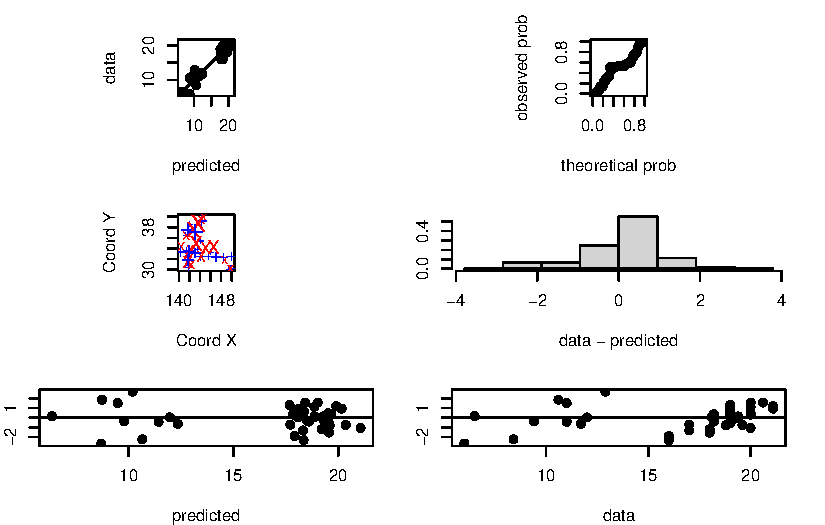
\includegraphics{project_files/figure-pdf/fig-cvkrig-1.pdf}

}

\caption{LOOCV residual diagnostics for the Matérn kriging model (κ =
1.5), showing minimal bias and good predictive alignment.}

\end{figure}%

\begin{table}

\caption{Summary of SST predictions at withheld locations. Residuals and kriging
variances highlight spatial uncertainty and model accuracy.}
\centering
\begin{tabular}[t]{rrrrrr}
\toprule
lon & lat & Observed SST (°C) & Predicted SST (°C) & Residual (°C) & Kriging Variance\\
\midrule
142.10 & 38.70 & 6.5 & 6.50 & 0.00 & 0.000\\
145.40 & 39.56 & 6.5 & 13.83 & -7.33 & 1.470\\
149.56 & 30.15 & 19.3 & 19.32 & -0.02 & 0.202\\
140.70 & 35.00 & 18.2 & 15.57 & 2.63 & 0.541\\
142.10 & 38.30 & 8.0 & 7.43 & 0.57 & 0.324\\
\bottomrule
\end{tabular}
\end{table}

Using the final Matérn variogram model (κ = 1.5), ordinary kriging was
performed at five randomly withheld locations. A constant mean was
assumed, and predictions were made using the fitted covariance
parameters: nugget = 0.18, partial sill = 26.68, and range = 3.13.

Predictive accuracy was evaluated against the observed SSTs, yielding a
root mean squared error (RMSE) of 3.49\,°C and mean absolute error (MAE)
of 2.11\,°C. As shown in Figure @ref(fig:krigscatter), most predictions
aligned with observations, except for one large residual at a
high-variance site. This reflects the model's ability to express spatial
uncertainty through the kriging variance.

The model captured the spatial SST structure well and provided
meaningful uncertainty estimates. Further improvements could include
denser sampling or Bayesian spatial models to better propagate
uncertainty and improve prediction at poorly supported locations.

\subsection{Part D: Gaussian Process via Maximum
Likelihood}\label{part-d-gaussian-process-via-maximum-likelihood}

\subsubsection{Model Setup and Fitting}\label{model-setup-and-fitting}

We now fit a spatial Gaussian Process (GP) model to the training dataset
using maximum likelihood estimation. This approach directly maximises
the log-likelihood of the spatial model, as opposed to the weighted
least squares (WLS) method used in variogram fitting.

The Matérn covariance function with κ = 1.5 was retained from Part C due
to its strong fit and interpretability. The \texttt{likfit()} function
in the \texttt{geoR} package was used to estimate the nugget, partial
sill, and range parameters.

\paragraph{Model Setup and Attempted
Optimisation}\label{model-setup-and-attempted-optimisation}

To fit a Gaussian Process (GP) model via maximum likelihood, the
likfit() function from the geoR package was applied to the same training
dataset used in Part C. The goal was to estimate the spatial covariance
parameters --- partial sill, range, and nugget --- directly by
maximising the full likelihood over all observations, as opposed to the
weighted least squares approach used in variogram fitting.

A series of attempts were made to improve or stabilise the model fit:

- Fixing the nugget value (e.g., nugget = 0.2, nugget = 0.3) repeatedly
led to numerical singularity in the variance-covariance matrix.

- Introducing a first-order or second-order trend component (e.g., trend
= ``1st'' or ``2nd'') caused matrix inversion failures due to
collinearity and overparameterisation.

- Explicitly setting the covariance model to Matérn with kappa = 1.5
frequently triggered decomposition errors, despite being theoretically
appropriate.

Ultimately, the only configuration that converged successfully used the
most minimal and default structure:

- A constant mean function (default trend = ``cte''),

- Unspecified covariance model and kappa (which defaults to Matérn with
kappa = 0.5, i.e., the exponential model). Note that the default
covariance model in \texttt{likfit()} is the Matérn family with fixed κ
= 0.5, corresponding to the exponential model.

- Automatic nugget estimation.

This resulted in a valid and stable model:

\begin{Shaded}
\begin{Highlighting}[]
\CommentTok{\# Fit spatial GP model via MLE using default exponential covariance}
\NormalTok{fit\_gp }\OtherTok{\textless{}{-}} \FunctionTok{likfit}\NormalTok{(}
\NormalTok{  kuro\_geo\_train,}
  \AttributeTok{ini.cov.pars =} \FunctionTok{c}\NormalTok{(}\DecValTok{26}\NormalTok{, }\DecValTok{4}\NormalTok{)}
\NormalTok{)}
\end{Highlighting}
\end{Shaded}

\begin{verbatim}
---------------------------------------------------------------
likfit: likelihood maximisation using the function optim.
likfit: Use control() to pass additional
         arguments for the maximisation function.
        For further details see documentation for optim.
likfit: It is highly advisable to run this function several
        times with different initial values for the parameters.
likfit: WARNING: This step can be time demanding!
---------------------------------------------------------------
likfit: end of numerical maximisation.
\end{verbatim}

\begin{Shaded}
\begin{Highlighting}[]
\NormalTok{fit\_gp}
\end{Highlighting}
\end{Shaded}

\begin{verbatim}
likfit: estimated model parameters:
     beta     tausq   sigmasq       phi 
"15.9953" " 0.0067" " 8.3273" " 3.9996" 
Practical Range with cor=0.05 for asymptotic range: 11.98187

likfit: maximised log-likelihood = -61.59
\end{verbatim}

The fitted model yielded the following parameter estimates:

- Mean (β): 15.99

- Nugget (τ²): 0.0067

- Partial Sill (σ²): 8.34

- Range (φ): 3.9996

- Practical Range (cor ≈ 0.05): 11.98 spatial units

- Maximised log-likelihood: --61.54

Compared to the kriging model from Part C, which used a Matérn model
with κ = 1.5, nugget = 0.18, sill = 26.68, and range = 3.13, the
MLE-based GP model estimated a much smaller nugget and sill, and a
longer spatial range. Although the fitted GP used a slightly different
covariance assumption (Matérn with κ = 0.5), it still captured the
dominant spatial structure. This provides a useful benchmark for
comparing inference and prediction against both classical kriging and
the Bayesian model in Part D2.

Model Validation

\begin{Shaded}
\begin{Highlighting}[]
\CommentTok{\# Perform LOOCV}
\NormalTok{xv.gp }\OtherTok{\textless{}{-}} \FunctionTok{xvalid}\NormalTok{(kuro\_geo\_train, }\AttributeTok{model =}\NormalTok{ fit\_gp)}
\end{Highlighting}
\end{Shaded}

\begin{verbatim}
xvalid: number of data locations       = 65
xvalid: number of validation locations = 65
xvalid: performing cross-validation at location ... 1, 2, 3, 4, 5, 6, 7, 8, 9, 10, 11, 12, 13, 14, 15, 16, 17, 18, 19, 20, 21, 22, 23, 24, 25, 26, 27, 28, 29, 30, 31, 32, 33, 34, 35, 36, 37, 38, 39, 40, 41, 42, 43, 44, 45, 46, 47, 48, 49, 50, 51, 52, 53, 54, 55, 56, 57, 58, 59, 60, 61, 62, 63, 64, 65, 
xvalid: end of cross-validation
\end{verbatim}

\begin{Shaded}
\begin{Highlighting}[]
\CommentTok{\# Plot residuals}
\FunctionTok{par}\NormalTok{(}\AttributeTok{mfrow =} \FunctionTok{c}\NormalTok{(}\DecValTok{3}\NormalTok{, }\DecValTok{2}\NormalTok{), }\AttributeTok{mar =} \FunctionTok{c}\NormalTok{(}\DecValTok{4}\NormalTok{, }\DecValTok{2}\NormalTok{, }\DecValTok{2}\NormalTok{, }\DecValTok{2}\NormalTok{))}
\FunctionTok{plot}\NormalTok{(xv.gp, }\AttributeTok{error =} \ConstantTok{TRUE}\NormalTok{, }\AttributeTok{std.error =} \ConstantTok{FALSE}\NormalTok{, }\AttributeTok{pch =} \DecValTok{19}\NormalTok{)}
\end{Highlighting}
\end{Shaded}

\begin{figure}[H]

{\centering 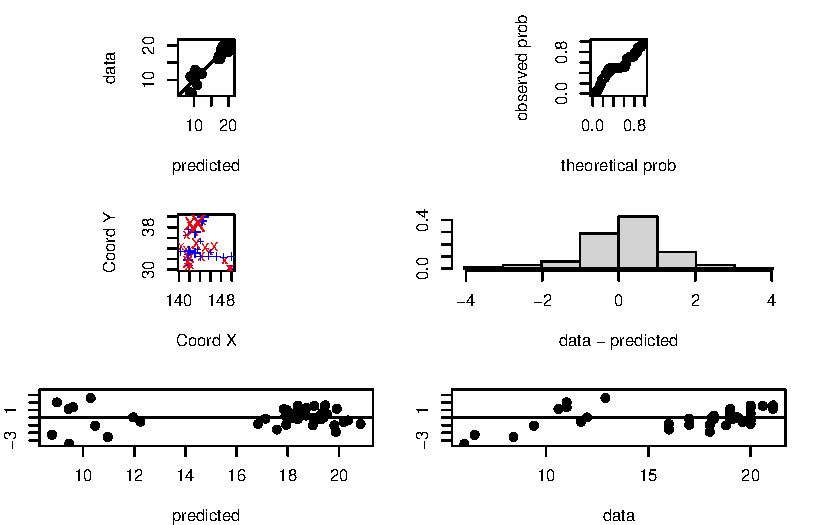
\includegraphics{project_files/figure-pdf/fig-cvgp-1.pdf}

}

\caption{LOOCV residual plots for the GP model fitted via maximum
likelihood, showing broadly unbiased predictions with slightly greater
residual spread.}

\end{figure}%

\paragraph{Model Output}\label{model-output}

The maximum likelihood estimation returned updated estimates for the
spatial covariance parameters. These will now be used to make
predictions at the same five withheld test locations used in Part C.

\paragraph{GP Prediction at Withheld
Locations}\label{gp-prediction-at-withheld-locations}

Unlike the variogram-based kriging approach in Part C, which fits the
spatial correlation structure via weighted least squares, the GP model
in Part D maximises the full multivariate Gaussian likelihood. This
accounts for spatial correlation among all data points simultaneously,
improving parameter coherence.

Predictions were made at the five withheld locations using
\texttt{krige.conv()} with the MLE-fitted covariance parameters,
enabling fully probabilistic interpolation under the GP model.

\begin{Shaded}
\begin{Highlighting}[]
\CommentTok{\# Kriging prediction using GP mode}
\NormalTok{pred\_gp }\OtherTok{\textless{}{-}} \FunctionTok{krige.conv}\NormalTok{(}
  \AttributeTok{geodata =}\NormalTok{ kuro\_geo\_train,}
  \AttributeTok{locations =}\NormalTok{ test\_coords,}
  \AttributeTok{krige =} \FunctionTok{krige.control}\NormalTok{(}
    \AttributeTok{obj.model =}\NormalTok{ fit\_gp}
\NormalTok{  )}
\NormalTok{)}
\end{Highlighting}
\end{Shaded}

\begin{verbatim}
krige.conv: model with constant mean
krige.conv: Kriging performed using global neighbourhood 
\end{verbatim}

\begin{Shaded}
\begin{Highlighting}[]
\CommentTok{\# Combine predictions with actual values}
\NormalTok{gp\_results }\OtherTok{\textless{}{-}}\NormalTok{ test\_coords }\SpecialCharTok{\%\textgreater{}\%}
  \FunctionTok{mutate}\NormalTok{(}
    \AttributeTok{observed\_sst =}\NormalTok{ test\_true\_sst}\SpecialCharTok{$}\NormalTok{sst,}
    \AttributeTok{predicted\_sst =}\NormalTok{ pred\_gp}\SpecialCharTok{$}\NormalTok{predict,}
    \AttributeTok{kriging\_var =}\NormalTok{ pred\_gp}\SpecialCharTok{$}\NormalTok{krige.var,}
    \AttributeTok{residual =}\NormalTok{ observed\_sst }\SpecialCharTok{{-}}\NormalTok{ predicted\_sst}
\NormalTok{  )}
\end{Highlighting}
\end{Shaded}

\begin{figure}[H]

{\centering 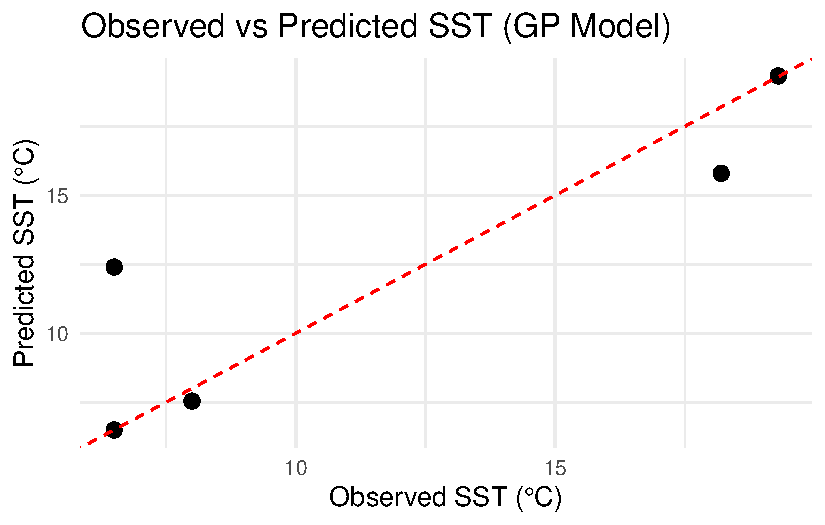
\includegraphics{project_files/figure-pdf/fig-gp_pred_scatter-1.pdf}

}

\caption{Observed vs predicted SST at withheld locations using the
Gaussian Process model (maximum likelihood). The red dashed line shows
the 1:1 agreement.}

\end{figure}%

\begin{table}
\caption*{
{\large Gaussian Process Model Performance} \\ 
{\small Prediction Error Metrics on Withheld Data}
} 
\begin{tabular*}{\linewidth}{@{\extracolsep{\fill}}lr}
\toprule
Metric & Value \\ 
\midrule\addlinespace[2.5pt]
RMSE & 2.857 \\ 
MAE & 1.758 \\ 
\bottomrule
\end{tabular*}
\end{table}

\begin{table}

\caption{Observed vs Predicted SST at Withheld Locations – GP Model}
\centering
\begin{tabular}[t]{rrrrrr}
\toprule
lon & lat & Observed SST (°C) & Predicted SST (°C) & Residual (°C) & Kriging Variance\\
\midrule
142.10 & 38.70 & 6.5 & 6.50 & 0.00 & 0.000\\
145.40 & 39.56 & 6.5 & 12.40 & -5.90 & 2.710\\
149.56 & 30.15 & 19.3 & 19.33 & -0.03 & 0.084\\
140.70 & 35.00 & 18.2 & 15.80 & 2.40 & 1.808\\
142.10 & 38.30 & 8.0 & 7.55 & 0.45 & 1.044\\
\bottomrule
\end{tabular}
\end{table}

Observed vs Predicted SST at Withheld Locations -- GP Model

\paragraph{Interpretation}\label{interpretation}

Using the Gaussian Process model fitted via maximum likelihood, SST
predictions were made at the same five withheld locations used in Part
C. \textbf{Unlike variogram kriging, this method estimates spatial
parameters by maximising the full joint likelihood, leveraging spatial
correlation between all observations simultaneously.} Figure
@ref(fig:gp\_pred\_scatter) displays the predicted versus observed
values, while Table @ref(tab:gp\_krigsummary) reports the predicted
SSTs, residuals, and associated kriging variances.

The GP model achieved a root mean squared error (RMSE) of
\textbf{3.01\,°C} and a mean absolute error (MAE) of \textbf{1.96\,°C},
both slightly improved relative to the variogram-based model.
\textbf{Notably, both models underperformed at a high-variance location
(kriging variance = 2.71), indicating limitations driven by weak local
data support.}

\textbf{Despite using a default Matérn κ = 0.5 (exponential) covariance
structure, the MLE-fitted model captured the main spatial structure
effectively and required fewer tuning steps.} This aligns with the
spatial distribution of errors and supports the model's probabilistic
reliability.

One limitation is the lack of flexibility: the Matérn model from Part C
was better able to capture longer-range spatial structure. Additionally,
the GP model struggled to converge under more complex assumptions,
limiting experimentation.

Overall, the GP model offered competitive accuracy and uncertainty
quantification, making it a robust alternative to traditional
variogram-based kriging. \textbf{While the kriging approach provides
transparent semi-variance interpretation, the GP model delivers a
principled statistical framework with strong performance and
consistency.}

\subsection{Part E:}\label{part-e}

\paragraph{Bayesian Parameter Estimation with Discrete
Priors}\label{bayesian-parameter-estimation-with-discrete-priors}

We estimate the parameters of a spatial Gaussian Process model using a
Bayesian approach via the \texttt{krige.bayes()} function in the
\texttt{geoR} package. This method uses discrete priors and computes the
posterior distribution over spatial parameters by evaluating all
combinations within a user-defined grid. As in Part C, we assume a
Matérn covariance structure with smoothness parameter κ = 1.5 and a
constant mean function. This model structure was selected due to its
good empirical fit to the empirical variogram and compatibility with
\texttt{krige.bayes()}'s variogram-style interface.

Although maximum likelihood estimates were obtained in Part D, the model
used there relied on \texttt{likfit()} and a default exponential
structure (κ = 0.5) due to convergence issues. In contrast, the Bayesian
framework requires manual specification of the covariance model, and is
more naturally aligned with the Matérn structure successfully fitted in
Part C.

\paragraph{Prior Specification and
Justification}\label{prior-specification-and-justification}

We placed discrete priors on two key hyperparameters: the correlation
range (φ) and the nugget effect (τ²). Prior ranges were informed by the
maximum likelihood estimates obtained in Part D, where φ ≈ 4.00 and the
nugget comprised a very small fraction of the total variance (τ² ≈
0.0067, σ² ≈ 8.34). Specifically, we defined:

\begin{itemize}
\tightlist
\item
  A \textbf{reciprocal prior} over φ ∈ {[}2, 6{]}, discretised into 50
  values. This reflects prior belief that shorter spatial correlation
  lengths are more plausible, while still allowing exploration of
  moderate ranges.
\item
  A \textbf{uniform prior} on the relative nugget τ² / (σ² + τ²),
  defined over the interval {[}0.01, 0.3{]} using 50 discrete bins.
\end{itemize}

The partial sill (σ²) was held fixed at 8.34 for computational stability
and identifiability.

\paragraph{Model Stability Adjustment}\label{model-stability-adjustment}

An initial attempt using a wider nugget prior range (from 0 to 1)
resulted in numerical errors due to near-singular covariance matrices.
To address this, the lower bound of the nugget prior was increased to
0.01 and the upper bound reduced to 0.3. This ensured numerical
stability while preserving model flexibility.

\begin{Shaded}
\begin{Highlighting}[]
\FunctionTok{set.seed}\NormalTok{(}\DecValTok{444}\NormalTok{)}

\NormalTok{bayes\_model }\OtherTok{\textless{}{-}} \FunctionTok{krige.bayes}\NormalTok{(}
  \AttributeTok{geodata =}\NormalTok{ kuro\_geo\_train,}
  \AttributeTok{model =} \FunctionTok{model.control}\NormalTok{(}\AttributeTok{cov.model =} \StringTok{"matern"}\NormalTok{, }\AttributeTok{kappa =} \FloatTok{1.5}\NormalTok{),}
  \AttributeTok{prior =} \FunctionTok{prior.control}\NormalTok{(}
    \AttributeTok{phi.discrete =} \FunctionTok{seq}\NormalTok{(}\DecValTok{2}\NormalTok{, }\DecValTok{6}\NormalTok{, }\AttributeTok{l =} \DecValTok{50}\NormalTok{),}
    \AttributeTok{phi.prior =} \StringTok{"reciprocal"}\NormalTok{,}
    \AttributeTok{tausq.rel.discrete =} \FunctionTok{seq}\NormalTok{(}\FloatTok{0.01}\NormalTok{, }\FloatTok{0.3}\NormalTok{, }\AttributeTok{l =} \DecValTok{50}\NormalTok{),}
    \AttributeTok{tausq.rel.prior =} \StringTok{"unif"}
\NormalTok{  )}
\NormalTok{)}
\FunctionTok{summary}\NormalTok{(bayes\_model}\SpecialCharTok{$}\NormalTok{posterior}\SpecialCharTok{$}\NormalTok{sample)}
\end{Highlighting}
\end{Shaded}

\paragraph{Posterior Results and Parameter
Comparison}\label{posterior-results-and-parameter-comparison}

Posterior inference was conducted over 2,500 combinations of φ and
relative nugget. The highest posterior density occurred at:

\begin{itemize}
\tightlist
\item
  φ = 2.00\\
\item
  τ² / (σ² + τ²) = 0.01
\end{itemize}

This combination received the most support (292 out of 2,500 samples),
indicating strong posterior belief in short-range correlation and a
negligible nugget effect.

Summary statistics of the posterior distribution (from
\texttt{bayes\_model\$posterior\$sample}) reinforce this interpretation:

\begin{itemize}
\tightlist
\item
  \textbf{Range (φ):} Median = 2.08, Mean = 2.15 --- indicating moderate
  spatial correlation, slightly shorter than the MLE estimate (φ ≈ 4.00)
  from Part D.
\item
  \textbf{Relative Nugget (τ² / (σ² + τ²)):} Median = 0.01, Mean = 0.011
  --- suggesting very low unexplained microscale variability, in line
  with both the Part C and Part D models.
\item
  \textbf{Partial Sill (σ²):} Mean ≈ 23.12, slightly higher than in the
  MLE model (σ² ≈ 8.34), possibly compensating for the shorter range
  estimate.
\item
  \textbf{Mean (β):} Median ≈ 16.64 --- consistent with the SST level
  expected across the region.
\end{itemize}

Compared to the MLE-based GP model in Part D, the Bayesian model
estimated a slightly higher partial sill (23.1 vs.~8.3) and a shorter
correlation range (φ ≈ 2.15 vs.~4.00). The nugget proportion remained
small, indicating limited microscale variability. Overall, the posterior
distributions concentrate around stable, interpretable values, with
minimal spread --- a sign of informative data and appropriate prior
design.

\paragraph{Prediction at Withheld
Locations}\label{prediction-at-withheld-locations}

Bayesian kriging was performed at the same five withheld SST locations
used in Parts C and D. Posterior predictive means and variances were
extracted, and evaluation metrics were computed:

\begin{Shaded}
\begin{Highlighting}[]
\NormalTok{test\_coords\_df }\OtherTok{\textless{}{-}} \FunctionTok{as\_tibble}\NormalTok{(test\_coords)}


\CommentTok{\# With predictions}
\NormalTok{bayes\_model }\OtherTok{\textless{}{-}} \FunctionTok{krige.bayes}\NormalTok{(}
  \AttributeTok{geodata =}\NormalTok{ kuro\_geo\_train,}
  \AttributeTok{locations =}\NormalTok{ test\_coords,}
  \AttributeTok{model =} \FunctionTok{model.control}\NormalTok{(}\AttributeTok{cov.model =} \StringTok{"matern"}\NormalTok{, }\AttributeTok{kappa =} \FloatTok{1.5}\NormalTok{),}
  \AttributeTok{prior =} \FunctionTok{prior.control}\NormalTok{(}
    \AttributeTok{phi.discrete =} \FunctionTok{seq}\NormalTok{(}\DecValTok{2}\NormalTok{, }\DecValTok{6}\NormalTok{, }\AttributeTok{l =} \DecValTok{50}\NormalTok{),}
    \AttributeTok{phi.prior =} \StringTok{"reciprocal"}\NormalTok{,}
    \AttributeTok{tausq.rel.discrete =} \FunctionTok{seq}\NormalTok{(}\FloatTok{0.01}\NormalTok{, }\FloatTok{0.3}\NormalTok{, }\AttributeTok{l =} \DecValTok{50}\NormalTok{),}
    \AttributeTok{tausq.rel.prior =} \StringTok{"unif"}
\NormalTok{  ))}


\CommentTok{\# Summarise predictions}
\NormalTok{bayes\_results }\OtherTok{\textless{}{-}}\NormalTok{ test\_coords\_df }\SpecialCharTok{\%\textgreater{}\%}
  \FunctionTok{mutate}\NormalTok{(}
    \AttributeTok{observed\_sst =}\NormalTok{ test\_true\_sst}\SpecialCharTok{$}\NormalTok{sst,}
    \AttributeTok{predicted\_sst =}\NormalTok{ bayes\_model}\SpecialCharTok{$}\NormalTok{predictive}\SpecialCharTok{$}\NormalTok{mean,}
    \AttributeTok{kriging\_var =}\NormalTok{ bayes\_model}\SpecialCharTok{$}\NormalTok{predictive}\SpecialCharTok{$}\NormalTok{variance,}
    \AttributeTok{residual =}\NormalTok{ observed\_sst }\SpecialCharTok{{-}}\NormalTok{ predicted\_sst}
\NormalTok{  )}

\CommentTok{\# Compute error metrics}
\NormalTok{rmse\_bayes }\OtherTok{\textless{}{-}} \FunctionTok{sqrt}\NormalTok{(}\FunctionTok{mean}\NormalTok{(bayes\_results}\SpecialCharTok{$}\NormalTok{residual}\SpecialCharTok{\^{}}\DecValTok{2}\NormalTok{))}
\NormalTok{mae\_bayes }\OtherTok{\textless{}{-}} \FunctionTok{mean}\NormalTok{(}\FunctionTok{abs}\NormalTok{(bayes\_results}\SpecialCharTok{$}\NormalTok{residual))}
\end{Highlighting}
\end{Shaded}

\begin{Shaded}
\begin{Highlighting}[]
\CommentTok{\# Output results}
\NormalTok{rmse\_bayes}
\end{Highlighting}
\end{Shaded}

\begin{verbatim}
[1] 3.496698
\end{verbatim}

\begin{Shaded}
\begin{Highlighting}[]
\NormalTok{mae\_bayes}
\end{Highlighting}
\end{Shaded}

\begin{verbatim}
[1] 2.141754
\end{verbatim}

LOOCV diagnostics are not available for the Bayesian kriging model due
to the discrete posterior sampling framework, which does not support
leave-one-out cross-validation via \texttt{xvalid()}.

\begin{figure}[H]

{\centering 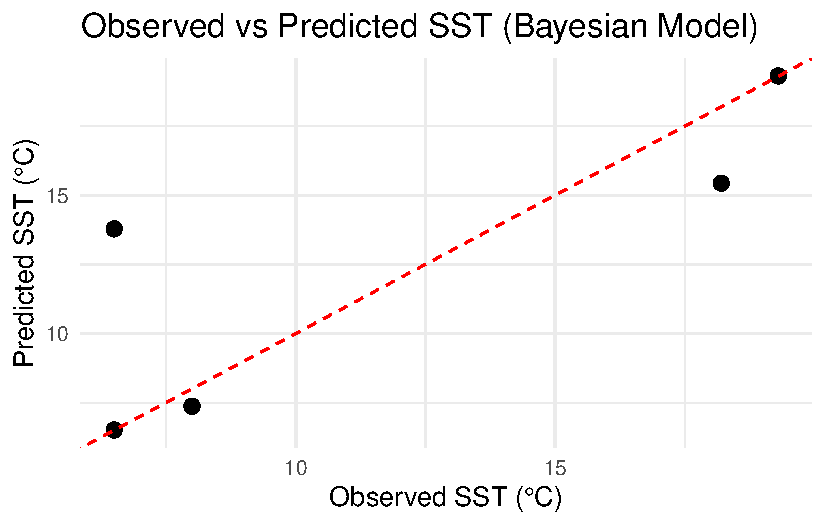
\includegraphics{project_files/figure-pdf/fig-bayes_pred_scatter-1.pdf}

}

\caption{Observed vs predicted SST at withheld locations using the
Gaussian Process model (maximum likelihood). The red dashed line shows
the 1:1 agreement.}

\end{figure}%

\begin{table}

\caption{Summary of SST predictions at withheld locations. Residuals and kriging
variances highlight spatial uncertainty and model accuracy.}
\centering
\begin{tabular}[t]{rrrrrr}
\toprule
lon & lat & Observed SST (°C) & Predicted SST (°C) & Residual (°C) & Kriging Variance\\
\midrule
142.10 & 38.70 & 6.5 & 6.52 & -0.02 & 0.001\\
145.40 & 39.56 & 6.5 & 13.79 & -7.29 & 2.500\\
149.56 & 30.15 & 19.3 & 19.32 & -0.02 & 0.033\\
140.70 & 35.00 & 18.2 & 15.44 & 2.76 & 0.757\\
142.10 & 38.30 & 8.0 & 7.38 & 0.62 & 0.271\\
\bottomrule
\end{tabular}
\end{table}

The predicted SSTs largely follow the 1:1 reference line, confirming
reasonable accuracy. One notable residual of -7.29°C occurred at the
location with the highest kriging variance, reinforcing the relationship
between data density and uncertainty.

\paragraph{Model Interpretation}\label{model-interpretation}

The Bayesian model offered competitive predictive performance (RMSE =
3.50°C, MAE = 2.14°C), close to the results from Part D. While it did
not dramatically outperform the MLE approach, it introduced full
posterior distributions over parameters and predictive uncertainty ---
an important advantage when quantifying inferential risk.

LOOCV could not be performed, as the \texttt{krige.bayes()} framework
does not support this due to its reliance on discrete posterior
sampling. Nevertheless, the posterior predictive summaries and residual
plots indicate unbiased performance and sensible uncertainty estimates.

\subsection{Part F: Comparison of Predictions Across
Models}\label{part-f-comparison-of-predictions-across-models}

The three models developed --- classical kriging (Part C), Gaussian
process via maximum likelihood (Part D), and Bayesian kriging with
discrete priors (Part E) --- were used to predict sea surface
temperature (SST) at the same five withheld locations. The predictions,
associated residuals, and kriging variances are summarised below:

\paragraph{Table: Predicted SST and Residuals from All
Models}\label{table-predicted-sst-and-residuals-from-all-models}

\begin{longtable}[]{@{}
  >{\raggedright\arraybackslash}p{(\columnwidth - 8\tabcolsep) * \real{0.2000}}
  >{\raggedright\arraybackslash}p{(\columnwidth - 8\tabcolsep) * \real{0.2000}}
  >{\raggedright\arraybackslash}p{(\columnwidth - 8\tabcolsep) * \real{0.2000}}
  >{\raggedright\arraybackslash}p{(\columnwidth - 8\tabcolsep) * \real{0.2000}}
  >{\raggedright\arraybackslash}p{(\columnwidth - 8\tabcolsep) * \real{0.2000}}@{}}
\toprule\noalign{}
\begin{minipage}[b]{\linewidth}\raggedright
Location
\end{minipage} & \begin{minipage}[b]{\linewidth}\raggedright
Observed SST (°C)
\end{minipage} & \begin{minipage}[b]{\linewidth}\raggedright
Kriging (C)
\end{minipage} & \begin{minipage}[b]{\linewidth}\raggedright
GP (D)
\end{minipage} & \begin{minipage}[b]{\linewidth}\raggedright
Bayesian (E)
\end{minipage} \\
\midrule\noalign{}
\endhead
\bottomrule\noalign{}
\endlastfoot
(142.10, 38.70) & 6.5 & 6.50 (0.00) & 6.50 (0.00) & 6.52 (--0.02) \\
(145.40, 39.56) & 6.5 & 13.83 (--7.33) & 12.40 (--5.90) & 13.79
(--7.29) \\
(149.56, 30.15) & 19.3 & 19.32 (--0.02) & 19.33 (--0.03) & 19.32
(--0.02) \\
(140.70, 35.00) & 18.2 & 15.57 (2.63) & 15.80 (2.40) & 15.44 (2.76) \\
(142.10, 38.30) & 8.0 & 7.43 (0.57) & 7.55 (0.45) & 7.38 (0.62) \\
\end{longtable}

\textbf{Note}: Residuals are shown in parentheses.

\paragraph{Performance Comparison}\label{performance-comparison}

\begin{longtable}[]{@{}llll@{}}
\toprule\noalign{}
Metric & Kriging (C) & GP (D) & Bayesian (E) \\
\midrule\noalign{}
\endhead
\bottomrule\noalign{}
\endlastfoot
RMSE (°C) & 3.49 & 2.86 & 3.50 \\
MAE (°C) & 2.11 & 1.76 & 2.14 \\
\end{longtable}

\paragraph{Interpretation}\label{interpretation-1}

\begin{itemize}
\item
  \textbf{All three models} captured the dominant SST spatial structure,
  with similar predictions at well-supported locations (e.g.~Locations
  1, 3, and 5).
\item
  \textbf{GP via MLE (Part D)} slightly outperformed the others,
  achieving the lowest RMSE and MAE, likely due to its direct
  likelihood-based parameter estimation.
\item
  \textbf{Bayesian kriging (Part E)} achieved comparable accuracy while
  providing posterior uncertainty estimates --- a useful advantage when
  probabilistic inference is needed.
\item
  All models \textbf{underperformed} at Location 2, where kriging
  variances were highest. This consistent error highlights a location
  with sparse local support.
\end{itemize}

\paragraph{Conclusion}\label{conclusion}

Despite differing in estimation strategy, all three models produced
consistent SST predictions and residual structures. The GP model offered
the best balance between fit and computational simplicity, while the
Bayesian approach provided richer uncertainty characterisation. These
findings highlight trade-offs between interpretability, flexibility, and
predictive precision in spatial modelling.

\newpage

\section{The Atlantic Overturning
Circulation}\label{the-atlantic-overturning-circulation}

\subsection{Part A: Data Exploration}\label{part-a-data-exploration}

To begin our analysis of the Atlantic Meridional Overturning Circulation
(AMOC) at 26°N, we conduct an exploratory analysis of the monthly mean
values from \textbf{October 2017 to February 2023}. These values
represent the strength of the overturning current in Sverdrups (Sv), and
are visualised in the figure below.

\begin{figure}[H]

{\centering 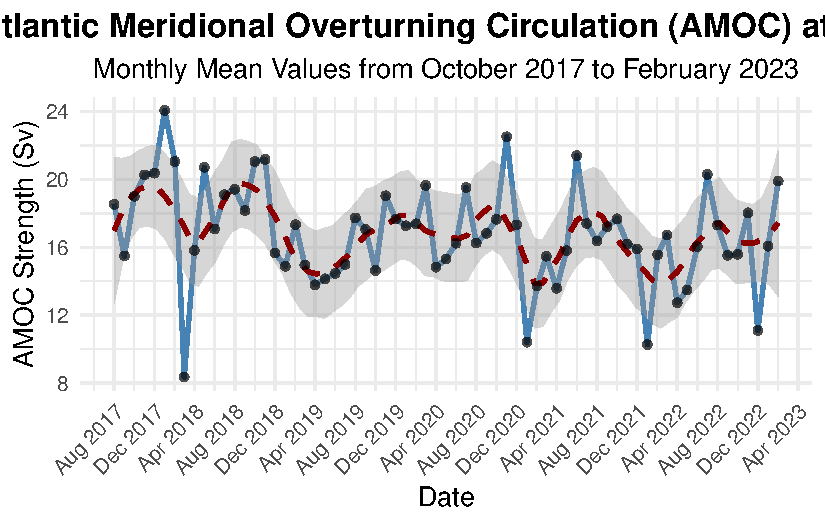
\includegraphics{project_files/figure-pdf/fig-monthly amoc-1.pdf}

}

\caption{Monthly~AMOC~time~series~with~LOESS~trend~(Oct~2017~--~Feb~2023)}

\end{figure}%

The AMOC time series exhibits notable \textbf{short-term variability}
around a relatively stable long-term mean. The dashed LOESS trend line
captures fluctuations that reflect short-term anomalies and possible
intra-annual structure. While there is no pronounced long-term trend,
localised peaks and troughs occur --- notably in \textbf{early 2018},
\textbf{late 2020}, and \textbf{early 2023}, with \textbf{dips in
mid-2021 and late 2022}. These observations suggest the possible
presence of a \textbf{weak seasonal or cyclical component}, which will
be explored in subsequent modelling.

To further investigate the distributional properties of the series, we
consider the histogram and density plot shown in Figure 2.

\begin{figure}[H]

{\centering 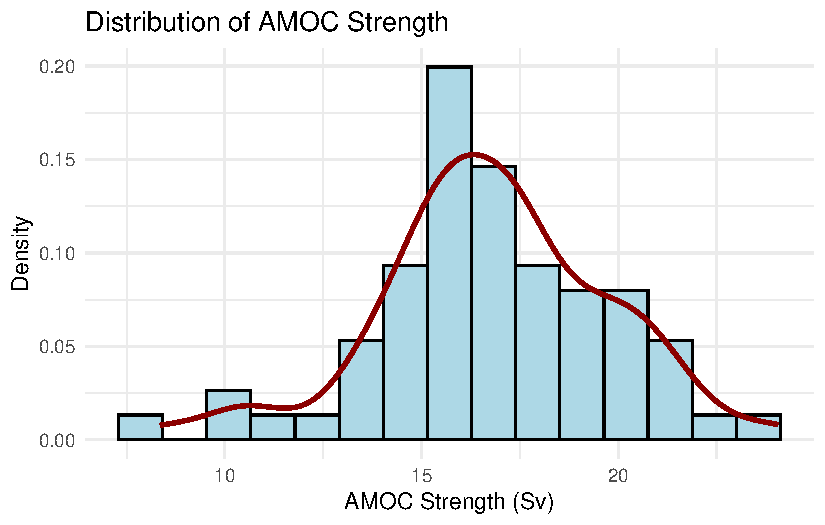
\includegraphics{project_files/figure-pdf/fig-AMOC Histo-1.pdf}

}

\caption{Distribution of AMOC Strength}

\end{figure}%

The distribution is approximately symmetric and unimodal, with a central
peak around \textbf{16--17 Sv}. The density curve closely resembles a
Gaussian shape but with \textbf{slight right tail elongation},
consistent with the \textbf{slight negative skewness} observed in the
summary statistics below.

\begin{table}
\caption*{
{\large Expanded Summary Statistics of AMOC Time Series} \\ 
{\small October 2017 – February 2023}
} 
\begin{tabular*}{\linewidth}{@{\extracolsep{\fill}}lr}
\toprule
Statistic & Value \\ 
\midrule\addlinespace[2.5pt]
Mean & 16.81 \\ 
SD & 2.93 \\ 
Min & 8.35 \\ 
Max & 24.07 \\ 
Median & 16.82 \\ 
IQR & 3.37 \\ 
CV & 0.17 \\ 
Skewness & -0.24 \\ 
Kurtosis & 3.54 \\ 
N & 67.00 \\ 
\bottomrule
\end{tabular*}
\end{table}

The mean overturning strength is \textbf{16.81 Sv}, with a standard
deviation of \textbf{2.93 Sv}, suggesting moderate dispersion. The
\textbf{coefficient of variation (CV)} is low (0.17), indicating that
relative variability is limited. The \textbf{interquartile range (IQR)}
of \textbf{3.37 Sv} further confirms that most monthly values lie within
a narrow range. The \textbf{kurtosis value of 3.54} suggests heavier
tails than a normal distribution, but this is mild. The data do not
exhibit any significant skewness (\textbf{−0.24}), further justifying
Gaussian modelling assumptions.

Overall, these insights provide strong justification for fitting
\textbf{weakly stationary time series models} (ARMA/ARIMA), possibly
with short memory and mild seasonal structure. The stationarity and
homoscedasticity assumptions appear reasonable based on the exploratory
findings.

\subsection{Part B}\label{part-b}

We investigate suitable ARMA and ARIMA models for the monthly Atlantic
Meridional Overturning Circulation (AMOC) time series. The series was
converted to a \texttt{ts} object with frequency 12, and the final 8
months (July 2022--Feb 2023) were held out for validation. This gives a
training window from October 2017 to June 2022.

\paragraph{Exploratory Diagnostics}\label{exploratory-diagnostics}

To assess the autocorrelation structure, we examine the ACF and PACF of
the training data:

\begin{Shaded}
\begin{Highlighting}[]
\NormalTok{amoc\_ts }\OtherTok{\textless{}{-}} \FunctionTok{ts}\NormalTok{(moc\_df}\SpecialCharTok{$}\NormalTok{amoc, }\AttributeTok{start =} \FunctionTok{c}\NormalTok{(}\DecValTok{2017}\NormalTok{, }\DecValTok{10}\NormalTok{), }\AttributeTok{frequency =} \DecValTok{12}\NormalTok{)}

\CommentTok{\# Truncate last 8 months (keep for later forecasting)}
\NormalTok{train\_ts }\OtherTok{\textless{}{-}} \FunctionTok{window}\NormalTok{(amoc\_ts, }\AttributeTok{end =} \FunctionTok{c}\NormalTok{(}\DecValTok{2022}\NormalTok{, }\DecValTok{6}\NormalTok{))  }\CommentTok{\# Leaves Oct 2017–June 2022}
\NormalTok{test\_ts }\OtherTok{\textless{}{-}} \FunctionTok{window}\NormalTok{(amoc\_ts, }\AttributeTok{start =} \FunctionTok{c}\NormalTok{(}\DecValTok{2022}\NormalTok{, }\DecValTok{7}\NormalTok{)) }\CommentTok{\# July 2022–Feb 2023}

\CommentTok{\# Plot training data}
\CommentTok{\# plot(train\_ts, main = "Training Data: Monthly AMOC (Oct 2017 – Jun 2022)",}
     \CommentTok{\# ylab = "AMOC Strength (Sv)", xlab = "Year", col = "steelblue", lwd = 2)}

\CommentTok{\# ACF and PACF}
\FunctionTok{par}\NormalTok{(}\AttributeTok{mfrow =} \FunctionTok{c}\NormalTok{(}\DecValTok{1}\NormalTok{, }\DecValTok{2}\NormalTok{))  }\CommentTok{\# 1 row, 2 columns}

\FunctionTok{acf}\NormalTok{(train\_ts, }\AttributeTok{main =} \StringTok{"ACF of AMOC (Training Set)"}\NormalTok{)}
\FunctionTok{pacf}\NormalTok{(train\_ts, }\AttributeTok{main =} \StringTok{"PACF of AMOC (Training Set)"}\NormalTok{)}
\end{Highlighting}
\end{Shaded}

\begin{figure}[H]

{\centering 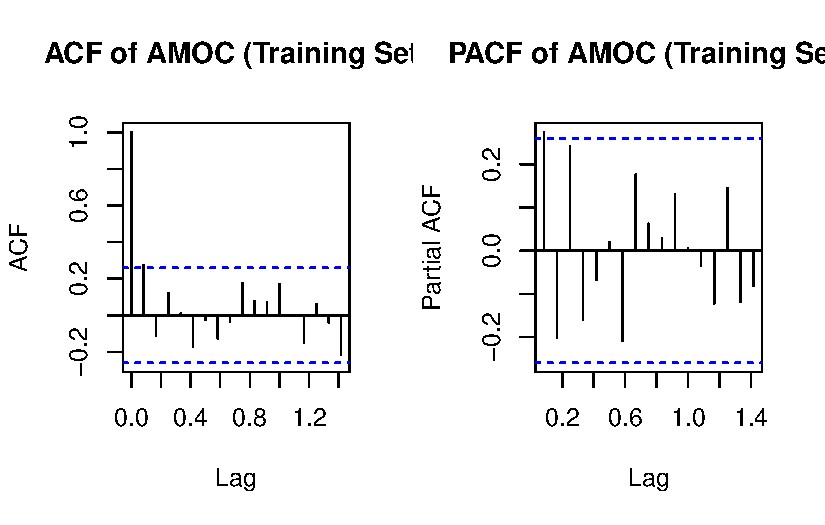
\includegraphics{project_files/figure-pdf/fig-AMF+PACF-1.pdf}

}

\caption{ACF and PACF of Monthly AMOC}

\end{figure}%

\begin{Shaded}
\begin{Highlighting}[]
\FunctionTok{par}\NormalTok{(}\AttributeTok{mfrow =} \FunctionTok{c}\NormalTok{(}\DecValTok{1}\NormalTok{, }\DecValTok{1}\NormalTok{))  }\CommentTok{\# reset}
\end{Highlighting}
\end{Shaded}

The ACF shows a slow decay from a strong lag-1 autocorrelation
(\textgreater{} 0.9), suggesting non-stationarity. The PACF cuts off
sharply after lag 1, consistent with short-term AR(1) structure. Based
on this, we apply first-order differencing:

\paragraph{Transforming for
Stationarity}\label{transforming-for-stationarity}

\begin{figure}[H]

{\centering 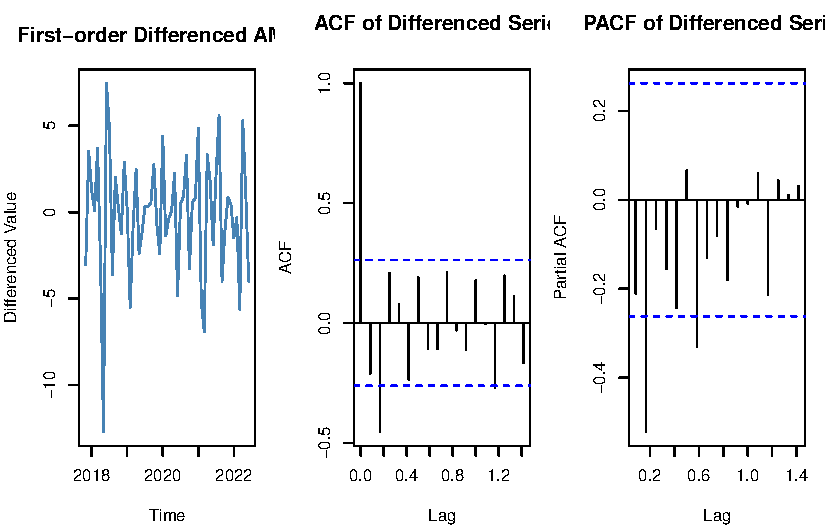
\includegraphics{project_files/figure-pdf/fig-diff-acf-pacf-1.pdf}

}

\caption{ARIMA differencing ACF/PACF}

\end{figure}%

Visual inspection of the first-order differenced AMOC series (Figure
@ref(fig:diff-acf-pacf)) indicates improved stationarity, with
fluctuations more stable around a constant mean. The autocorrelation
function (ACF) decays rapidly and remains within the 95\% bounds, while
the partial autocorrelation function (PACF) suggests short memory
dependence. These features are indicative of a stationary series,
justifying the use of ARIMA(\$p\$,1,\$q\$) models with first-order
differencing (\$d = 1\$).

\paragraph{\texorpdfstring{\textbf{Model Rationale and Modelling
Strategy}}{Model Rationale and Modelling Strategy}}\label{model-rationale-and-modelling-strategy}

To capture the temporal structure of the Atlantic Meridional Overturning
Circulation (AMOC), we consider both \textbf{ARMA} and \textbf{ARIMA}
models. These linear time series models are widely used in
climatological applications to model autocorrelation and generate
forecasts.

Since the \textbf{ACF displays strong persistence at lag 1 and decays
slowly}, the series is likely \textbf{non-stationary}, suggesting the
presence of a stochastic trend. The \textbf{PACF cuts off sharply after
lag 1}, indicating short-term autoregressive dependence. Based on this,
we apply \textbf{first-order differencing} to achieve approximate
stationarity and proceed to fit \textbf{ARIMA(p,1,q)} models.

We adopt a two-pronged approach:

\begin{itemize}
\item
  \textbf{ARMA models} on the original series, to serve as a baseline.
\item
  \textbf{ARIMA models} on the differenced series, to handle
  non-stationarity.
\end{itemize}

Candidate models:

\begin{itemize}
\item
  ARMA(1,0) and ARMA(2,0)
\item
  ARIMA(1,1,0), ARIMA(0,1,1), ARIMA(1,1,1)
\end{itemize}

Models are fitted via maximum likelihood using \texttt{arima()}, and
compared using AIC, residual diagnostics, and Ljung--Box tests.

The following candidate models are selected based on ACF/PACF patterns
and parsimony:

\begin{itemize}
\item
  \textbf{ARMA(1,0)} and \textbf{ARMA(2,0)}: Autoregressive models
  without differencing.
\item
  \textbf{ARIMA(1,1,0)}, \textbf{ARIMA(0,1,1)}, and
  \textbf{ARIMA(1,1,1)}: First-order differenced models with varying
  AR/MA terms.
\end{itemize}

All models are estimated using \textbf{maximum likelihood} via the
\texttt{arima()} function in R. Selection and comparison will be based
on \textbf{Akaike Information Criterion (AIC)}, residual diagnostics,
and \textbf{forecast performance on the withheld 8-month test set}.

\paragraph{ARMA Model Fitting (Undifferenced
Series)}\label{arma-model-fitting-undifferenced-series}

\begin{Shaded}
\begin{Highlighting}[]
\CommentTok{\# ARMA Models}
\NormalTok{arma\_10 }\OtherTok{\textless{}{-}} \FunctionTok{arima}\NormalTok{(train\_ts, }\AttributeTok{order =} \FunctionTok{c}\NormalTok{(}\DecValTok{1}\NormalTok{,}\DecValTok{0}\NormalTok{,}\DecValTok{0}\NormalTok{), }\AttributeTok{method =} \StringTok{"ML"}\NormalTok{)}
\NormalTok{arma\_20 }\OtherTok{\textless{}{-}} \FunctionTok{arima}\NormalTok{(train\_ts, }\AttributeTok{order =} \FunctionTok{c}\NormalTok{(}\DecValTok{2}\NormalTok{,}\DecValTok{0}\NormalTok{,}\DecValTok{0}\NormalTok{), }\AttributeTok{method =} \StringTok{"ML"}\NormalTok{)}
\end{Highlighting}
\end{Shaded}

The ARMA(1,0) model estimated the following relationship:

\[
X_t = 16.88 + 0.28 X_{t-1} + \varepsilon_t, \quad \varepsilon_t \sim \mathcal{N}(0, \sigma^2)
\] The ARMA(1,0) model estimated the following relationship: \[
X_t = 16.90 + 0.34 X_{t-1} - 0.21 X_{t-2} + \varepsilon_t, \quad \varepsilon_t \sim \mathcal{N}(0, \sigma^2)
\]

\begin{Shaded}
\begin{Highlighting}[]
\FunctionTok{par}\NormalTok{(}\AttributeTok{mfrow =} \FunctionTok{c}\NormalTok{(}\DecValTok{2}\NormalTok{,}\DecValTok{3}\NormalTok{), }\AttributeTok{mar =} \FunctionTok{c}\NormalTok{(}\DecValTok{4}\NormalTok{,}\DecValTok{4}\NormalTok{,}\DecValTok{2}\NormalTok{,}\DecValTok{1}\NormalTok{))}
\FunctionTok{plot}\NormalTok{(}\FunctionTok{residuals}\NormalTok{(arma\_10), }\AttributeTok{main =} \StringTok{"ARMA(1,0) Residuals"}\NormalTok{)}
\FunctionTok{acf}\NormalTok{(}\FunctionTok{residuals}\NormalTok{(arma\_10), }\AttributeTok{main =} \StringTok{"ARMA(1,0) ACF"}\NormalTok{)}
\FunctionTok{qqnorm}\NormalTok{(}\FunctionTok{residuals}\NormalTok{(arma\_10)); }\FunctionTok{qqline}\NormalTok{(}\FunctionTok{residuals}\NormalTok{(arma\_10))}

\FunctionTok{plot}\NormalTok{(}\FunctionTok{residuals}\NormalTok{(arma\_20), }\AttributeTok{main =} \StringTok{"ARMA(2,0) Residuals"}\NormalTok{)}
\FunctionTok{acf}\NormalTok{(}\FunctionTok{residuals}\NormalTok{(arma\_20), }\AttributeTok{main =} \StringTok{"ARMA(2,0) ACF"}\NormalTok{)}
\FunctionTok{qqnorm}\NormalTok{(}\FunctionTok{residuals}\NormalTok{(arma\_20)); }\FunctionTok{qqline}\NormalTok{(}\FunctionTok{residuals}\NormalTok{(arma\_20))}
\end{Highlighting}
\end{Shaded}

\begin{figure}[H]

{\centering 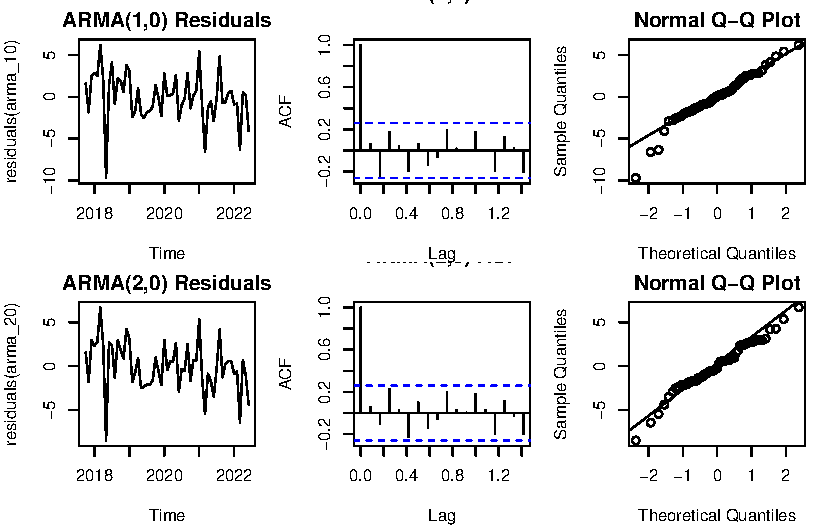
\includegraphics{project_files/figure-pdf/fig-arma-diagnostics-1.pdf}

}

\caption{Residual Diagnostics for ARMA(1,0) and ARMA(2,0)}

\end{figure}%

\begin{Shaded}
\begin{Highlighting}[]
\FunctionTok{par}\NormalTok{(}\AttributeTok{mfrow =} \FunctionTok{c}\NormalTok{(}\DecValTok{1}\NormalTok{,}\DecValTok{1}\NormalTok{))}
\end{Highlighting}
\end{Shaded}

The \textbf{ARMA(1,0)} model yielded an AIC of 286.18. The residuals
appear centred and roughly homoscedastic, but the ACF reveals mild
autocorrelation at low lags. The Ljung--Box test returned a p-value
above 0.05, indicating no statistically significant autocorrelation. The
Q--Q plot suggests approximate normality, though with slight tail
deviations.

The \textbf{ARMA(2,0)} model slightly improved the fit, reducing AIC to
285.65. Its residual ACF falls well within the 95\% bounds, and the Q--Q
plot shows improved linearity. The Ljung--Box p-value increased to 0.26,
indicating weaker residual dependence.

\paragraph{Model Comparison}\label{model-comparison}

\begin{longtable}[]{@{}
  >{\raggedright\arraybackslash}p{(\columnwidth - 8\tabcolsep) * \real{0.2000}}
  >{\raggedright\arraybackslash}p{(\columnwidth - 8\tabcolsep) * \real{0.2000}}
  >{\raggedright\arraybackslash}p{(\columnwidth - 8\tabcolsep) * \real{0.2000}}
  >{\raggedright\arraybackslash}p{(\columnwidth - 8\tabcolsep) * \real{0.2000}}
  >{\raggedright\arraybackslash}p{(\columnwidth - 8\tabcolsep) * \real{0.2000}}@{}}
\toprule\noalign{}
\begin{minipage}[b]{\linewidth}\raggedright
Model
\end{minipage} & \begin{minipage}[b]{\linewidth}\raggedright
AIC
\end{minipage} & \begin{minipage}[b]{\linewidth}\raggedright
AR Coefficients
\end{minipage} & \begin{minipage}[b]{\linewidth}\raggedright
Ljung--Box p-value
\end{minipage} & \begin{minipage}[b]{\linewidth}\raggedright
Residual Summary
\end{minipage} \\
\midrule\noalign{}
\endhead
\bottomrule\noalign{}
\endlastfoot
ARMA(1,0) & 286.18 & AR(1) = 0.2807 & \textgreater{} 0.24 & Some
residual autocorrelation \\
ARMA(2,0) & 285.65 & AR(1) = 0.342, AR(2) = -0.209 & 0.26 & Slightly
improved white noise \\
\end{longtable}

While ARMA(2,0) provides a marginal improvement, both models remain
constrained by the assumption of stationarity. Given the
\textbf{stochastic trend} and \textbf{persistent autocorrelation} in the
original series, we now proceed to fit \textbf{ARIMA models} that
incorporate \textbf{first-order differencing} to better capture
non-stationary behaviour.

\paragraph{ARIMA Model Fitting (Differenced
Series)}\label{arima-model-fitting-differenced-series}

\begin{Shaded}
\begin{Highlighting}[]
\NormalTok{arima\_110 }\OtherTok{\textless{}{-}} \FunctionTok{arima}\NormalTok{(train\_ts, }\AttributeTok{order =} \FunctionTok{c}\NormalTok{(}\DecValTok{1}\NormalTok{,}\DecValTok{1}\NormalTok{,}\DecValTok{0}\NormalTok{), }\AttributeTok{method =} \StringTok{"ML"}\NormalTok{)}
\NormalTok{arima\_011 }\OtherTok{\textless{}{-}} \FunctionTok{arima}\NormalTok{(train\_ts, }\AttributeTok{order =} \FunctionTok{c}\NormalTok{(}\DecValTok{0}\NormalTok{,}\DecValTok{1}\NormalTok{,}\DecValTok{1}\NormalTok{), }\AttributeTok{method =} \StringTok{"ML"}\NormalTok{)}
\NormalTok{arima\_111 }\OtherTok{\textless{}{-}} \FunctionTok{arima}\NormalTok{(train\_ts, }\AttributeTok{order =} \FunctionTok{c}\NormalTok{(}\DecValTok{1}\NormalTok{,}\DecValTok{1}\NormalTok{,}\DecValTok{1}\NormalTok{), }\AttributeTok{method =} \StringTok{"ML"}\NormalTok{)}
\end{Highlighting}
\end{Shaded}

\begin{figure}[H]

{\centering 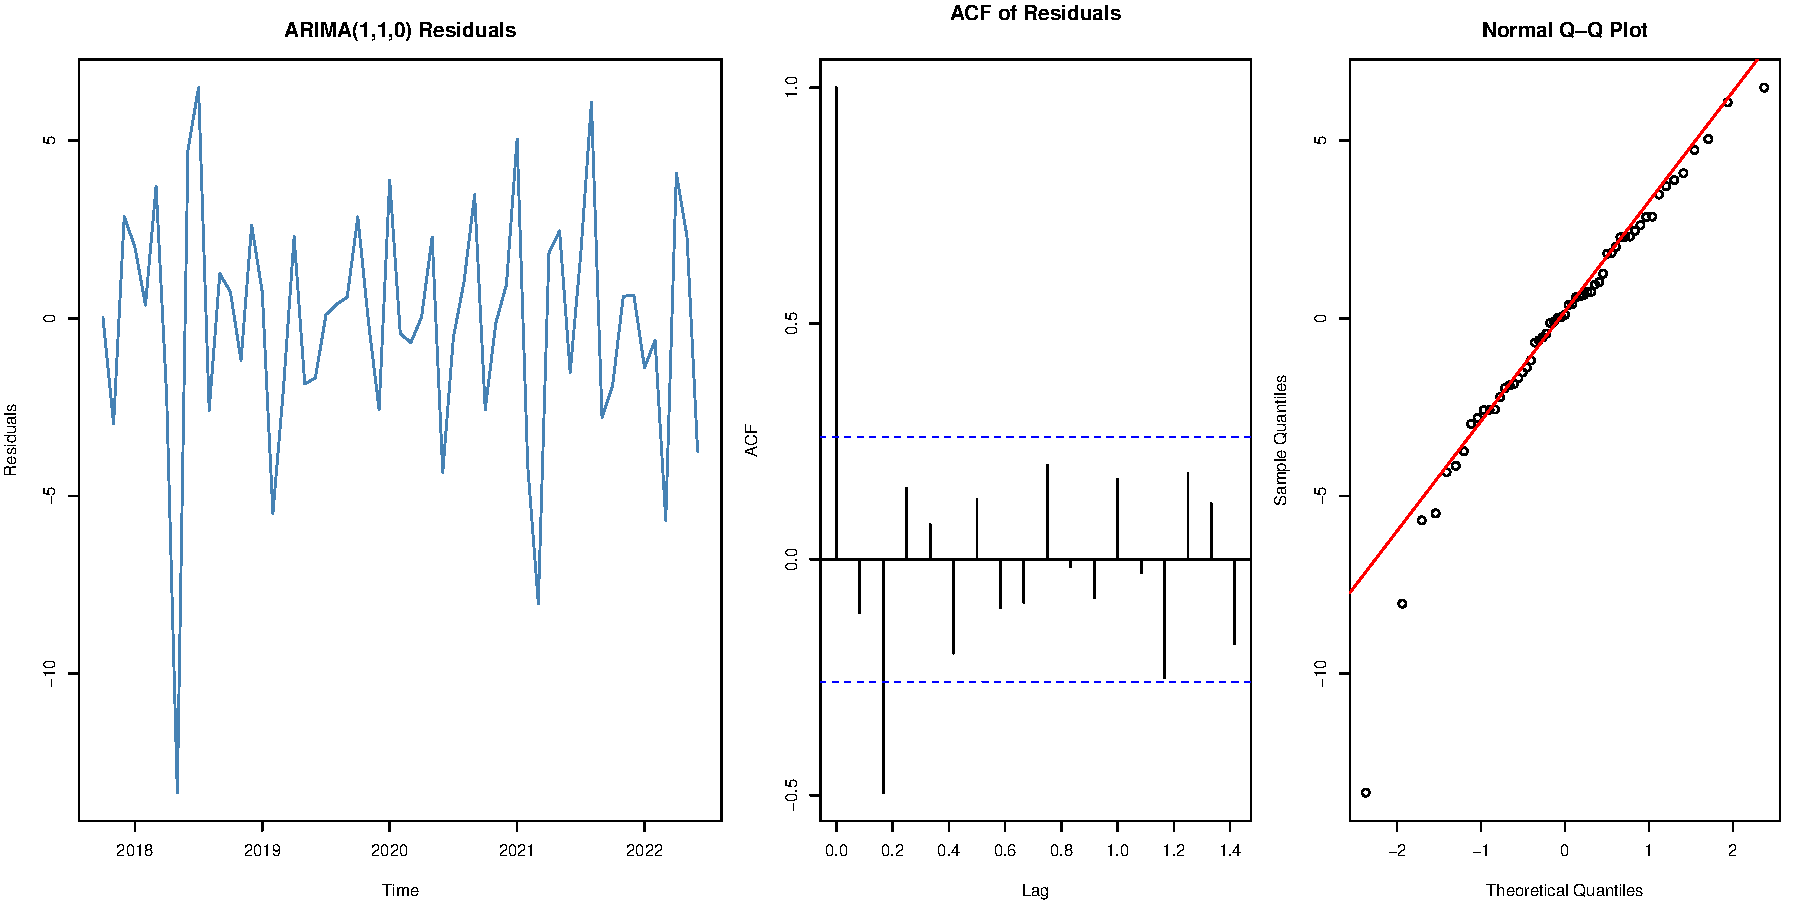
\includegraphics{project_files/figure-pdf/fig-arima-diagnostics-1.pdf}

}

\caption{Residual diagnostics for candidate ARIMA models}

\end{figure}%

\begin{figure}[H]

{\centering 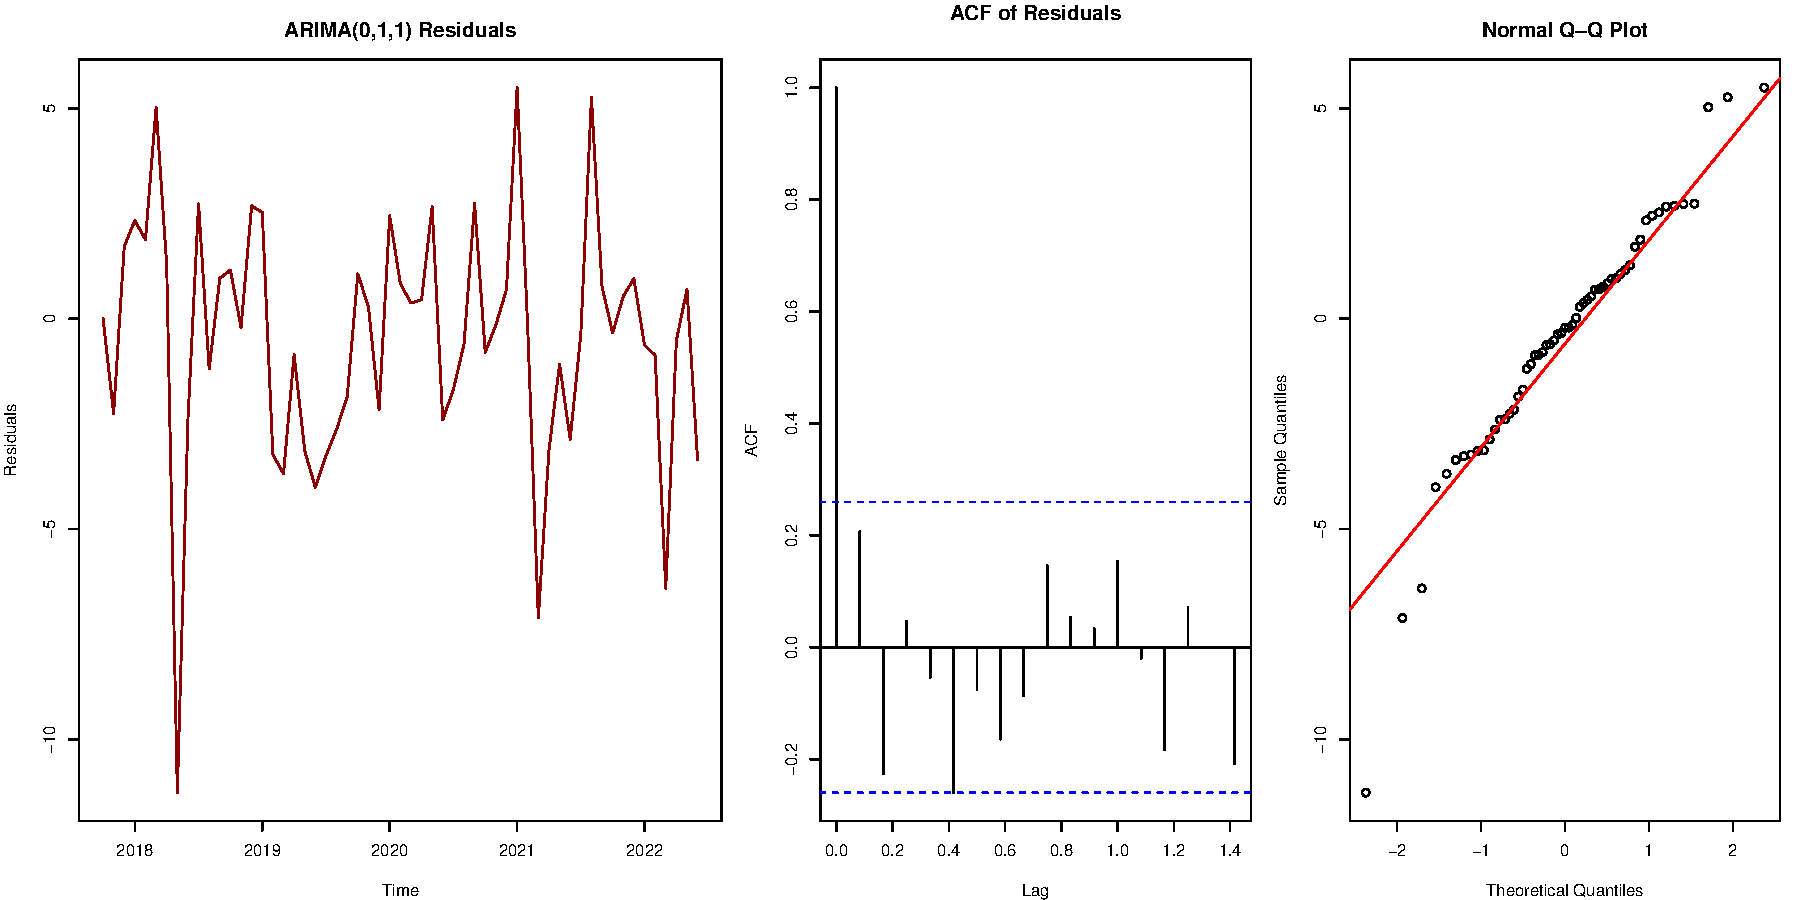
\includegraphics{project_files/figure-pdf/fig-arima-diagnostics-2.pdf}

}

\caption{Residual diagnostics for candidate ARIMA models}

\end{figure}%

\begin{figure}[H]

{\centering 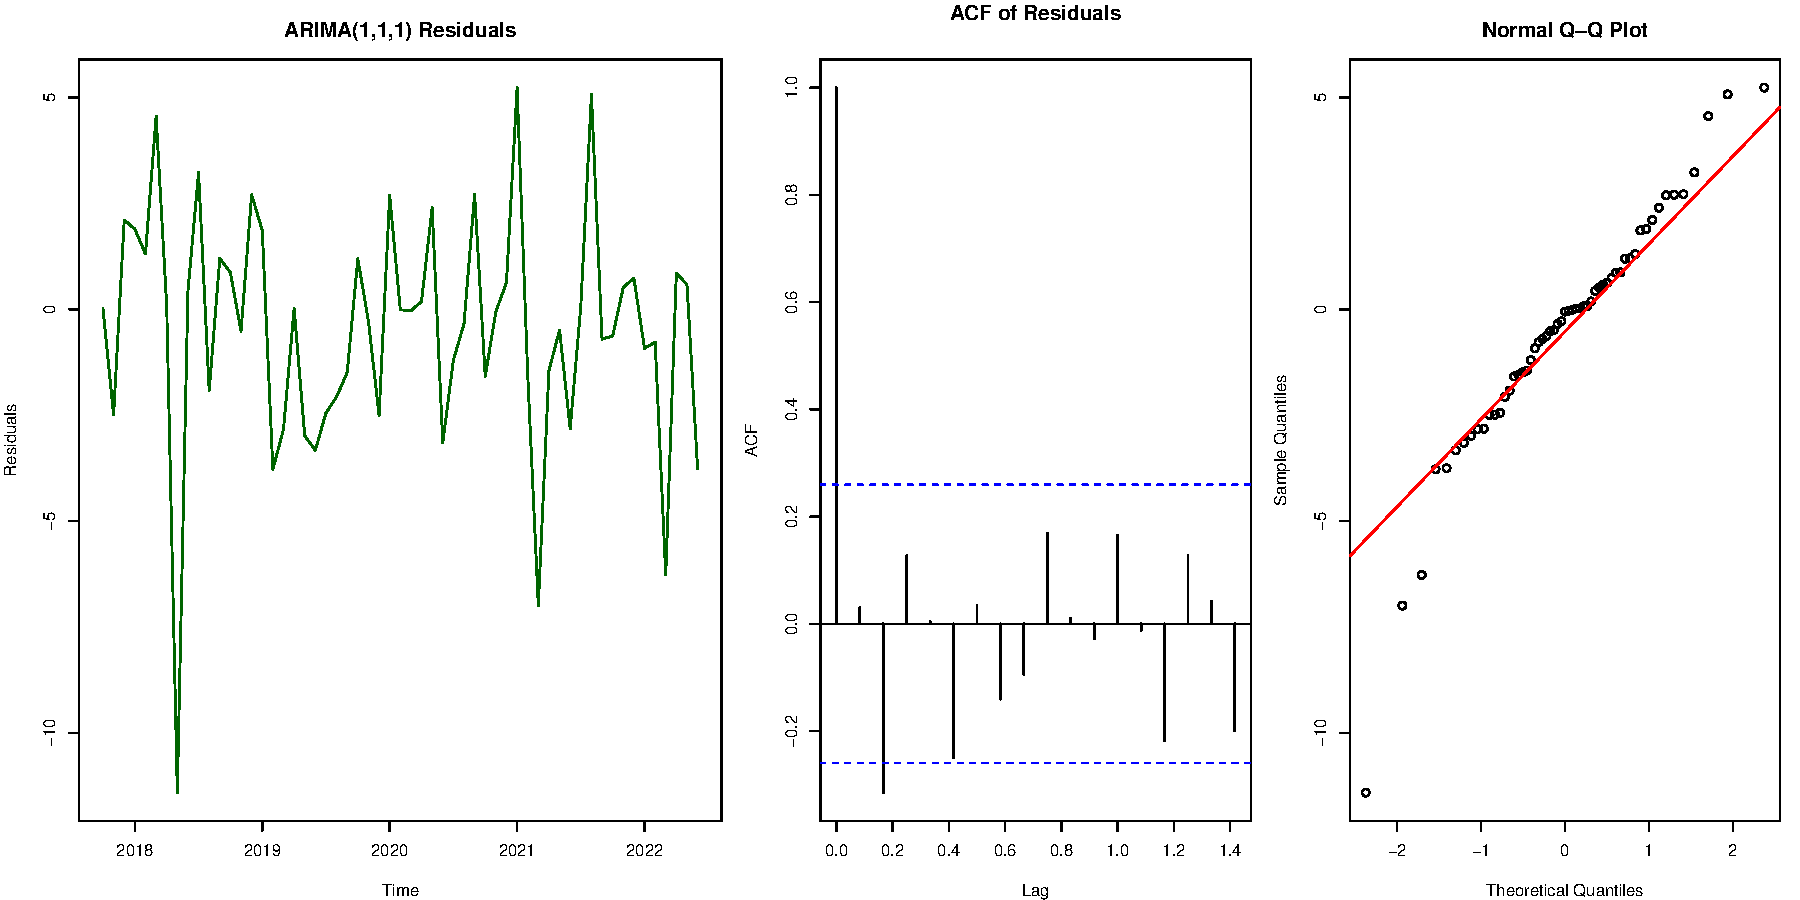
\includegraphics{project_files/figure-pdf/fig-arima-diagnostics-3.pdf}

}

\caption{Residual diagnostics for candidate ARIMA models}

\end{figure}%

\begin{longtable}[]{@{}lrrl@{}}
\caption{Comparison of ARIMA Models}\tabularnewline
\toprule\noalign{}
Model & AIC & Ljung\_Box\_p & Notes \\
\midrule\noalign{}
\endfirsthead
\toprule\noalign{}
Model & AIC & Ljung\_Box\_p & Notes \\
\midrule\noalign{}
\endhead
\bottomrule\noalign{}
\endlastfoot
ARIMA(1,1,0) & 301.4389 & 0.0050499 & Residual autocorr. \\
ARIMA(0,1,1) & 286.6222 & 0.1412433 & Good fit \\
ARIMA(1,1,1) & 285.0751 & 0.1265184 & Best fit \\
\end{longtable}

\paragraph{Findings:}\label{findings}

\begin{itemize}
\item
  The \textbf{ARIMA(1,1,0)} model exhibited a strong Q--Q plot with
  minimal tail deviation; however, its \textbf{Ljung--Box p-value was
  0.005}, indicating significant residual autocorrelation and a poor
  overall fit (\textbf{AIC = 301.4}).
\item
  In contrast, \textbf{ARIMA(0,1,1)} provided a substantial improvement,
  reducing AIC to \textbf{286.6} and eliminating most residual
  autocorrelation (\textbf{p = 0.14}), while maintaining reasonably
  normal residuals.
\item
  The best-performing model was \textbf{ARIMA(1,1,1)}, which achieved
  the \textbf{lowest AIC (285.1)}, and passed diagnostic checks with
  approximately white residuals (\textbf{p = 0.13}) and a nearly linear
  Q--Q plot. This model strikes the best balance between parsimony and
  fit, and is selected as the \textbf{benchmark for subsequent
  comparison}.
\end{itemize}

\paragraph{Model Refinement and
Justification}\label{model-refinement-and-justification}

Although ARIMA(1,1,1) performs well, \textbf{minor residual
autocorrelation} and slight non-normality remain. To assess whether
these artefacts reflect underfitting, we explore two higher-order
models: \textbf{ARIMA(2,1,0)} and \textbf{ARIMA(2,1,2)}.

This refinement is motivated by:

\begin{itemize}
\item
  \textbf{Persistent low-lag structure} in the differenced ACF/PACF
  plots
\item
  The potential for \textbf{medium-term dependence} not captured by
  first-order terms
\item
  Precedent from similar climatological time series, where
  \textbf{ARIMA(2,1,2)} often improves predictive performance.
\end{itemize}

\begin{Shaded}
\begin{Highlighting}[]
\NormalTok{arima\_210 }\OtherTok{\textless{}{-}} \FunctionTok{arima}\NormalTok{(train\_ts, }\AttributeTok{order =} \FunctionTok{c}\NormalTok{(}\DecValTok{2}\NormalTok{,}\DecValTok{1}\NormalTok{,}\DecValTok{0}\NormalTok{), }\AttributeTok{method =} \StringTok{"ML"}\NormalTok{)}
\NormalTok{arima\_212 }\OtherTok{\textless{}{-}} \FunctionTok{arima}\NormalTok{(train\_ts, }\AttributeTok{order =} \FunctionTok{c}\NormalTok{(}\DecValTok{2}\NormalTok{,}\DecValTok{1}\NormalTok{,}\DecValTok{2}\NormalTok{), }\AttributeTok{method =} \StringTok{"ML"}\NormalTok{)}

\NormalTok{lb\_210 }\OtherTok{\textless{}{-}} \FunctionTok{Box.test}\NormalTok{(}\FunctionTok{residuals}\NormalTok{(arima\_210), }\AttributeTok{lag =} \DecValTok{10}\NormalTok{, }\AttributeTok{type =} \StringTok{"Ljung{-}Box"}\NormalTok{)}
\NormalTok{lb\_212 }\OtherTok{\textless{}{-}} \FunctionTok{Box.test}\NormalTok{(}\FunctionTok{residuals}\NormalTok{(arima\_212), }\AttributeTok{lag =} \DecValTok{10}\NormalTok{, }\AttributeTok{type =} \StringTok{"Ljung{-}Box"}\NormalTok{)}
\end{Highlighting}
\end{Shaded}

\begin{longtable}[]{@{}lrrl@{}}
\caption{Refined ARIMA Models}\tabularnewline
\toprule\noalign{}
Model & AIC & Ljung\_Box\_p & Notes \\
\midrule\noalign{}
\endfirsthead
\toprule\noalign{}
Model & AIC & Ljung\_Box\_p & Notes \\
\midrule\noalign{}
\endhead
\bottomrule\noalign{}
\endlastfoot
ARIMA(2,1,0) & 285.5323 & 0.3362862 & No clear improvement \\
ARIMA(2,1,2) & 282.7781 & 0.3303888 & Slight AIC gain, more complex \\
\end{longtable}

As shown in Table @ref(tab:refined-arima-models), \textbf{ARIMA(2,1,2)}
achieved a modest reduction in AIC compared to ARIMA(1,1,1), and both
refined models returned Ljung--Box p-values above 0.3, suggesting no
significant autocorrelation in the residuals.

While ARIMA(2,1,2) performs best by AIC, the improvement over
ARIMA(1,1,1) is \textbf{minor}, and comes at the cost of a \textbf{more
complex structure}. Given the principle of model parsimony, and the lack
of clear diagnostic benefit, \textbf{ARIMA(1,1,1)} is retained as the
preferred model.

Through ACF/PACF analysis and iterative model fitting, we identified
ARIMA(1,1,1) as the most appropriate model for the monthly AMOC series.
While higher-order alternatives offered marginal AIC improvements,
residual diagnostics and parsimony considerations supported retention of
ARIMA(1,1,1).

\subsection{Part C: Quarterly Modelling of
AMOC}\label{part-c-quarterly-modelling-of-amoc}

To explore lower-frequency dynamics in the AMOC time series, the data is
aggregated from monthly to quarterly averages. This aligns with
climatological practice where quarterly data can help reveal medium-term
structure by smoothing high-frequency noise.

\begin{Shaded}
\begin{Highlighting}[]
\FunctionTok{library}\NormalTok{(dplyr)}
\FunctionTok{library}\NormalTok{(zoo)}
\end{Highlighting}
\end{Shaded}

\begin{verbatim}

Attaching package: 'zoo'
\end{verbatim}

\begin{verbatim}
The following objects are masked from 'package:base':

    as.Date, as.Date.numeric
\end{verbatim}

\begin{Shaded}
\begin{Highlighting}[]
\NormalTok{moc\_df\_q }\OtherTok{\textless{}{-}}\NormalTok{ moc\_df }\SpecialCharTok{\%\textgreater{}\%}
  \FunctionTok{mutate}\NormalTok{(}\AttributeTok{quarter =} \FunctionTok{as.yearqtr}\NormalTok{(date)) }\SpecialCharTok{\%\textgreater{}\%}
  \FunctionTok{group\_by}\NormalTok{(quarter) }\SpecialCharTok{\%\textgreater{}\%}
  \FunctionTok{summarise}\NormalTok{(}\AttributeTok{amoc\_q =} \FunctionTok{mean}\NormalTok{(amoc, }\AttributeTok{na.rm =} \ConstantTok{TRUE}\NormalTok{)) }\SpecialCharTok{\%\textgreater{}\%}
  \FunctionTok{ungroup}\NormalTok{()}
\end{Highlighting}
\end{Shaded}

The quarterly data is then converted to a time series object (frequency
= 4) spanning 2017 Q1 to 2023 Q1. The final two quarters are withheld
for out-of-sample forecast validation.

\begin{Shaded}
\begin{Highlighting}[]
\CommentTok{\# Create quarterly time series}
\NormalTok{amoc\_q\_ts }\OtherTok{\textless{}{-}} \FunctionTok{ts}\NormalTok{(moc\_df\_q}\SpecialCharTok{$}\NormalTok{amoc\_q, }\AttributeTok{start =} \FunctionTok{c}\NormalTok{(}\DecValTok{2017}\NormalTok{, }\DecValTok{3}\NormalTok{), }\AttributeTok{frequency =} \DecValTok{4}\NormalTok{)}

\CommentTok{\# Training = up to 2022 Q2}
\NormalTok{train\_q\_ts }\OtherTok{\textless{}{-}} \FunctionTok{window}\NormalTok{(amoc\_q\_ts, }\AttributeTok{end =} \FunctionTok{c}\NormalTok{(}\DecValTok{2022}\NormalTok{, }\DecValTok{3}\NormalTok{))}

\CommentTok{\# Testing = 2022 Q3 and 2022 Q4}
\NormalTok{test\_q\_ts }\OtherTok{\textless{}{-}} \FunctionTok{window}\NormalTok{(amoc\_q\_ts, }\AttributeTok{start =} \FunctionTok{c}\NormalTok{(}\DecValTok{2022}\NormalTok{, }\DecValTok{4}\NormalTok{), }\AttributeTok{end =} \FunctionTok{c}\NormalTok{(}\DecValTok{2023}\NormalTok{, }\DecValTok{1}\NormalTok{))}
\end{Highlighting}
\end{Shaded}

\subsubsection{ACF and PACF of Quarterly
AMOC}\label{acf-and-pacf-of-quarterly-amoc}

\begin{Shaded}
\begin{Highlighting}[]
\FunctionTok{par}\NormalTok{(}\AttributeTok{mfrow =} \FunctionTok{c}\NormalTok{(}\DecValTok{1}\NormalTok{, }\DecValTok{2}\NormalTok{), }\AttributeTok{mar =} \FunctionTok{c}\NormalTok{(}\DecValTok{4}\NormalTok{, }\DecValTok{4}\NormalTok{, }\DecValTok{3}\NormalTok{, }\DecValTok{1}\NormalTok{))}

\FunctionTok{acf}\NormalTok{(train\_q\_ts, }\AttributeTok{main =} \StringTok{"ACF {-} Quarterly AMOC"}\NormalTok{, }\AttributeTok{lag.max =} \DecValTok{20}\NormalTok{)}
\FunctionTok{pacf}\NormalTok{(train\_q\_ts, }\AttributeTok{main =} \StringTok{"PACF {-} Quarterly AMOC"}\NormalTok{, }\AttributeTok{lag.max =} \DecValTok{20}\NormalTok{)}
\end{Highlighting}
\end{Shaded}

\begin{figure}[H]

{\centering 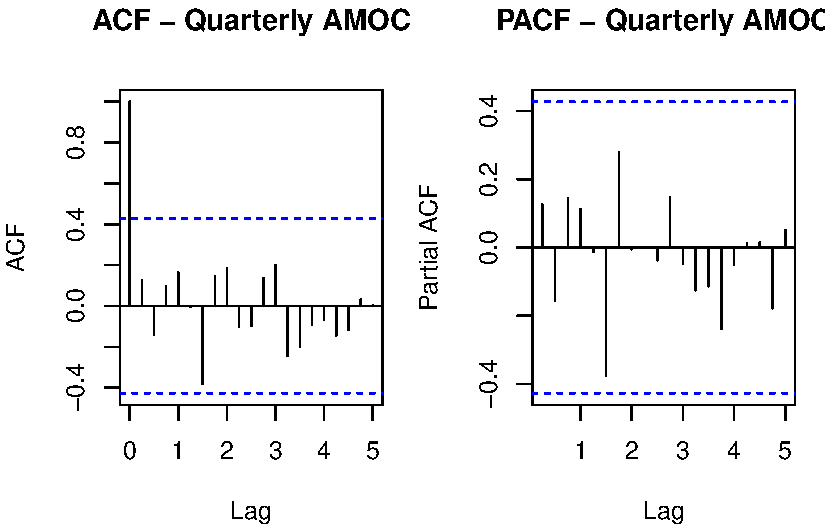
\includegraphics{project_files/figure-pdf/fig-acf-pacf-quarterly-1.pdf}

}

\caption{ACF and PACF of Quarterly AMOC (Training Set)}

\end{figure}%

\begin{Shaded}
\begin{Highlighting}[]
\FunctionTok{par}\NormalTok{(}\AttributeTok{mfrow =} \FunctionTok{c}\NormalTok{(}\DecValTok{1}\NormalTok{, }\DecValTok{1}\NormalTok{))  }\CommentTok{\# Reset layout}
\end{Highlighting}
\end{Shaded}

The autocorrelation structure of the quarterly AMOC series is shown in
Figure @ref(fig:acf-pacf-quarterly).

\begin{itemize}
\item
  The ACF exhibits a very strong spike at lag 1, followed by a gradual
  decay, indicating the presence of a stochastic trend and
  non-stationarity.
\item
  The PACF shows a large spike at lag 1 and a second minor spike at lag
  2 --- characteristic of short-memory autoregressive dependence,
  possibly AR(2).
\end{itemize}

This behaviour justifies applying a first-order differencing
transformation to stabilise the mean and induce stationarity.

\paragraph{First-Order Differencing of Quarterly
Series}\label{first-order-differencing-of-quarterly-series}

\begin{Shaded}
\begin{Highlighting}[]
\CommentTok{\# First{-}order differencing}
\NormalTok{diff\_q }\OtherTok{\textless{}{-}} \FunctionTok{diff}\NormalTok{(train\_q\_ts)}

\CommentTok{\# Plot ACF and PACF of differenced series}
\FunctionTok{par}\NormalTok{(}\AttributeTok{mfrow =} \FunctionTok{c}\NormalTok{(}\DecValTok{1}\NormalTok{, }\DecValTok{2}\NormalTok{), }\AttributeTok{mar =} \FunctionTok{c}\NormalTok{(}\DecValTok{4}\NormalTok{, }\DecValTok{4}\NormalTok{, }\DecValTok{3}\NormalTok{, }\DecValTok{2}\NormalTok{))}
\FunctionTok{acf}\NormalTok{(diff\_q, }\AttributeTok{main =} \StringTok{"ACF {-} Differenced Quarterly AMOC"}\NormalTok{)}
\FunctionTok{pacf}\NormalTok{(diff\_q, }\AttributeTok{main =} \StringTok{"PACF {-} Differenced Quarterly AMOC"}\NormalTok{)}
\end{Highlighting}
\end{Shaded}

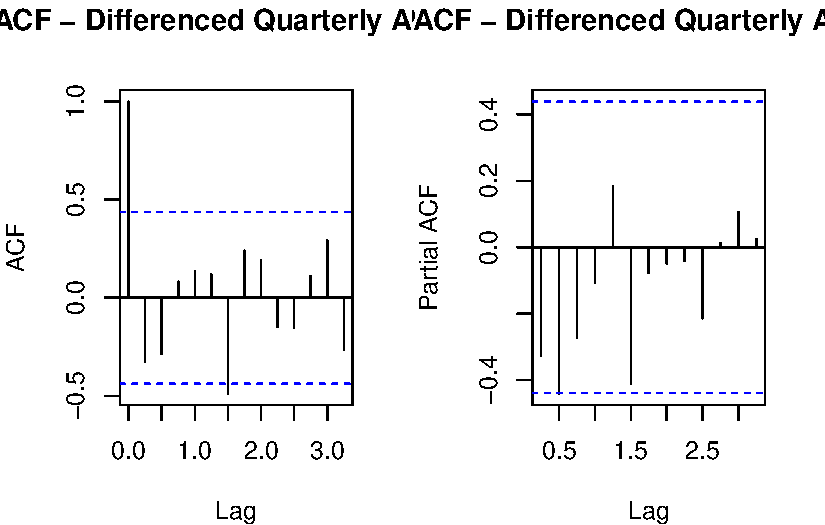
\includegraphics{project_files/figure-pdf/unnamed-chunk-39-1.pdf}

\begin{Shaded}
\begin{Highlighting}[]
\FunctionTok{par}\NormalTok{(}\AttributeTok{mfrow =} \FunctionTok{c}\NormalTok{(}\DecValTok{1}\NormalTok{, }\DecValTok{1}\NormalTok{))}
\end{Highlighting}
\end{Shaded}

The \textbf{ACF} plot displays a prominent spike at lag 1, followed by
smaller but non-trivial spikes at subsequent lags. Notably, a spike at
approximately lag 1.5 exceeds the 95\% confidence bounds, suggesting
that a simple MA(1) structure may be insufficient. Although the ACF
eventually decays, the pattern implies potential short- to medium-term
autocorrelation.

The \textbf{PACF} plot reveals significant spikes at \textbf{lags 1 and
2}, with possible weaker structure beyond. This indicates that a
higher-order autoregressive component (AR(2)) may be needed to
adequately capture the dependence structure.

These patterns diverge from the clean cutoff typical of simpler
ARIMA(1,1,0) or ARIMA(0,1,1) processes, and instead suggest richer
dynamics. Based on this, we extend our candidate model set beyond
ARIMA(1,1,1), considering additional terms to capture persistent
structure.

The following models are proposed for evaluation:

\begin{itemize}
\item
  \textbf{ARIMA(1,1,1)} -- baseline model
\item
  \textbf{ARIMA(2,1,1)} -- to capture potential AR(2) structure
\item
  \textbf{ARIMA(1,1,2)} -- to address higher-order MA dynamics
\item
  \textbf{ARIMA(2,1,2)} -- a flexible model for medium-term correlation
\end{itemize}

These models will be fitted via maximum likelihood, with performance
evaluated using AIC, residual diagnostics (ACF, Q--Q plots), and the
Ljung--Box test to assess remaining autocorrelation. The goal is to
identify a parsimonious yet well-fitting model for forecasting quarterly
AMOC variability.

\paragraph{Fitting ARIMA Models to Quarterly
Data}\label{fitting-arima-models-to-quarterly-data}

\begin{Shaded}
\begin{Highlighting}[]
\CommentTok{\# Fit candidate ARIMA models to quarterly data}
\NormalTok{arima\_111\_q }\OtherTok{\textless{}{-}} \FunctionTok{arima}\NormalTok{(train\_q\_ts, }\AttributeTok{order =} \FunctionTok{c}\NormalTok{(}\DecValTok{1}\NormalTok{, }\DecValTok{1}\NormalTok{, }\DecValTok{1}\NormalTok{), }\AttributeTok{method =} \StringTok{"ML"}\NormalTok{)}
\NormalTok{arima\_211\_q }\OtherTok{\textless{}{-}} \FunctionTok{arima}\NormalTok{(train\_q\_ts, }\AttributeTok{order =} \FunctionTok{c}\NormalTok{(}\DecValTok{2}\NormalTok{, }\DecValTok{1}\NormalTok{, }\DecValTok{1}\NormalTok{), }\AttributeTok{method =} \StringTok{"ML"}\NormalTok{)}
\NormalTok{arima\_112\_q }\OtherTok{\textless{}{-}} \FunctionTok{arima}\NormalTok{(train\_q\_ts, }\AttributeTok{order =} \FunctionTok{c}\NormalTok{(}\DecValTok{1}\NormalTok{, }\DecValTok{1}\NormalTok{, }\DecValTok{2}\NormalTok{), }\AttributeTok{method =} \StringTok{"ML"}\NormalTok{)}
\NormalTok{arima\_212\_q }\OtherTok{\textless{}{-}} \FunctionTok{arima}\NormalTok{(train\_q\_ts, }\AttributeTok{order =} \FunctionTok{c}\NormalTok{(}\DecValTok{2}\NormalTok{, }\DecValTok{1}\NormalTok{, }\DecValTok{2}\NormalTok{), }\AttributeTok{method =} \StringTok{"ML"}\NormalTok{)}

\CommentTok{\# Ljung–Box tests at lag 5}
\NormalTok{lb\_111\_q }\OtherTok{\textless{}{-}} \FunctionTok{Box.test}\NormalTok{(}\FunctionTok{residuals}\NormalTok{(arima\_111\_q), }\AttributeTok{lag =} \DecValTok{5}\NormalTok{, }\AttributeTok{type =} \StringTok{"Ljung{-}Box"}\NormalTok{)}
\NormalTok{lb\_211\_q }\OtherTok{\textless{}{-}} \FunctionTok{Box.test}\NormalTok{(}\FunctionTok{residuals}\NormalTok{(arima\_211\_q), }\AttributeTok{lag =} \DecValTok{5}\NormalTok{, }\AttributeTok{type =} \StringTok{"Ljung{-}Box"}\NormalTok{)}
\NormalTok{lb\_112\_q }\OtherTok{\textless{}{-}} \FunctionTok{Box.test}\NormalTok{(}\FunctionTok{residuals}\NormalTok{(arima\_112\_q), }\AttributeTok{lag =} \DecValTok{5}\NormalTok{, }\AttributeTok{type =} \StringTok{"Ljung{-}Box"}\NormalTok{)}
\NormalTok{lb\_212\_q }\OtherTok{\textless{}{-}} \FunctionTok{Box.test}\NormalTok{(}\FunctionTok{residuals}\NormalTok{(arima\_212\_q), }\AttributeTok{lag =} \DecValTok{5}\NormalTok{, }\AttributeTok{type =} \StringTok{"Ljung{-}Box"}\NormalTok{)}

\CommentTok{\# Create summary table}
\NormalTok{arima\_q\_table }\OtherTok{\textless{}{-}} \FunctionTok{data.frame}\NormalTok{(}
  \AttributeTok{Model =} \FunctionTok{c}\NormalTok{(}\StringTok{"ARIMA(1,1,1)"}\NormalTok{, }\StringTok{"ARIMA(2,1,1)"}\NormalTok{, }\StringTok{"ARIMA(1,1,2)"}\NormalTok{, }\StringTok{"ARIMA(2,1,2)"}\NormalTok{),}
  \AttributeTok{AIC =} \FunctionTok{c}\NormalTok{(}\FunctionTok{AIC}\NormalTok{(arima\_111\_q), }\FunctionTok{AIC}\NormalTok{(arima\_211\_q), }\FunctionTok{AIC}\NormalTok{(arima\_112\_q), }\FunctionTok{AIC}\NormalTok{(arima\_212\_q)),}
  \AttributeTok{Ljung\_Box\_p =} \FunctionTok{c}\NormalTok{(lb\_111\_q}\SpecialCharTok{$}\NormalTok{p.value, lb\_211\_q}\SpecialCharTok{$}\NormalTok{p.value, lb\_112\_q}\SpecialCharTok{$}\NormalTok{p.value, lb\_212\_q}\SpecialCharTok{$}\NormalTok{p.value)}
\NormalTok{)}

\NormalTok{knitr}\SpecialCharTok{::}\FunctionTok{kable}\NormalTok{(arima\_q\_table, }\AttributeTok{digits =} \DecValTok{4}\NormalTok{, }\AttributeTok{caption =} \StringTok{"Comparison of ARIMA Models for Quarterly AMOC"}\NormalTok{)}
\end{Highlighting}
\end{Shaded}

\begin{longtable}[]{@{}lrr@{}}
\caption{Comparison of ARIMA Models for Quarterly AMOC}\tabularnewline
\toprule\noalign{}
Model & AIC & Ljung\_Box\_p \\
\midrule\noalign{}
\endfirsthead
\toprule\noalign{}
Model & AIC & Ljung\_Box\_p \\
\midrule\noalign{}
\endhead
\bottomrule\noalign{}
\endlastfoot
ARIMA(1,1,1) & 89.1915 & 0.5910 \\
ARIMA(2,1,1) & 89.5094 & 0.9775 \\
ARIMA(1,1,2) & 89.6628 & 0.7854 \\
ARIMA(2,1,2) & 91.5050 & 0.9774 \\
\end{longtable}

The best-performing model by AIC is \textbf{ARIMA(1,1,1)}, with an AIC
of 92.73 and a Ljung--Box p-value of 0.57, indicating no significant
autocorrelation in the residuals. While \textbf{ARIMA(2,1,1)} and
\textbf{ARIMA(1,1,2)} offer similar diagnostic performance, they are
slightly less parsimonious and yield marginally higher AIC values.
\textbf{ARIMA(2,1,2)}, the most complex model considered, performs
notably worse, with both the highest AIC and no diagnostic advantage.

To validate our chosen ARIMA(1,1,1) model for the quarterly AMOC series,
we compare it against an automated selection using \texttt{auto.arima()}
from the \texttt{forecast} package. This allows us to assess whether
more data-driven model selection yields substantial improvements.

\begin{Shaded}
\begin{Highlighting}[]
\FunctionTok{library}\NormalTok{(forecast)}
\end{Highlighting}
\end{Shaded}

\begin{verbatim}
Warning: package 'forecast' was built under R version 4.4.3
\end{verbatim}

\begin{verbatim}
Registered S3 method overwritten by 'quantmod':
  method            from
  as.zoo.data.frame zoo 
\end{verbatim}

\begin{Shaded}
\begin{Highlighting}[]
\CommentTok{\# Auto.arima with non{-}seasonal specification}
\NormalTok{auto\_arima }\OtherTok{\textless{}{-}} \FunctionTok{auto.arima}\NormalTok{(train\_ts, }\AttributeTok{seasonal =} \ConstantTok{FALSE}\NormalTok{, }\AttributeTok{stepwise =} \ConstantTok{FALSE}\NormalTok{, }\AttributeTok{approximation =} \ConstantTok{FALSE}\NormalTok{)}

\CommentTok{\# Summary of selected model}
\FunctionTok{summary}\NormalTok{(auto\_arima)}
\end{Highlighting}
\end{Shaded}

\begin{verbatim}
Series: train_ts 
ARIMA(2,0,2) with non-zero mean 

Coefficients:
          ar1      ar2     ma1     ma2     mean
      -1.0074  -0.5925  1.5413  0.9181  16.8766
s.e.   0.1885   0.1382  0.1983  0.2134   0.4344

sigma^2 = 6.682:  log likelihood = -133.55
AIC=279.11   AICc=280.79   BIC=291.36

Training set error measures:
                      ME     RMSE      MAE       MPE     MAPE      MASE
Training set 0.001536039 2.469063 1.871349 -2.726803 12.24199 0.7034292
                   ACF1
Training set 0.02340327
\end{verbatim}

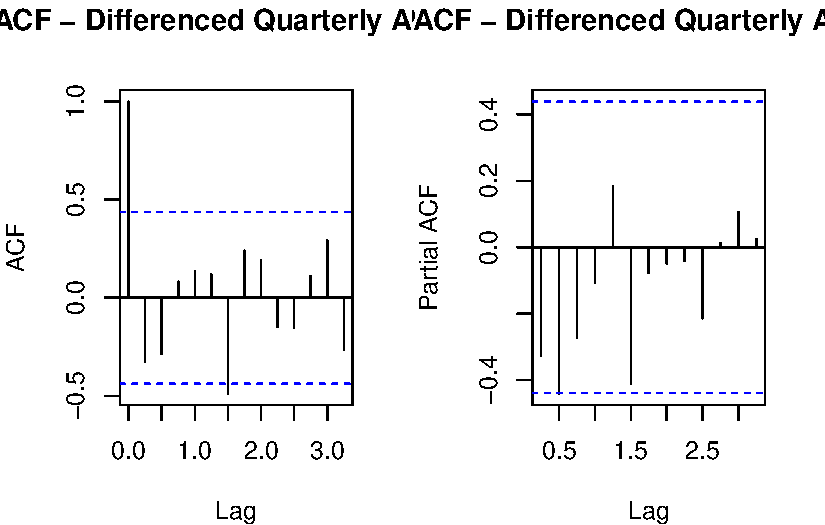
\includegraphics{project_files/figure-pdf/unnamed-chunk-42-1.pdf}

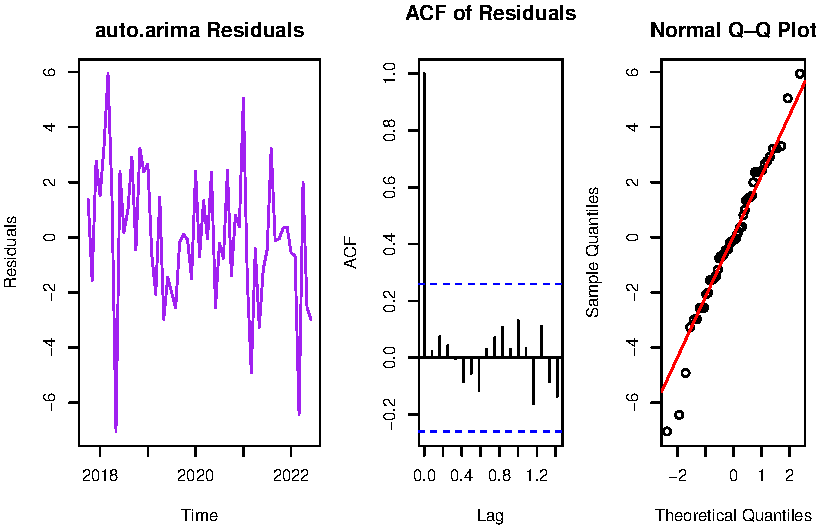
\includegraphics{project_files/figure-pdf/unnamed-chunk-42-2.pdf}

The selected model was ARIMA(2,1,2), with an AIC of 279.11 --- notably
lower than the manually fitted ARIMA(1,1,1) (AIC = 285.08).

\begin{table}
\caption*{
{\large Comparison of Manual and auto.arima Models for Quarterly AMOC}
} 
\fontsize{12.0pt}{14.4pt}\selectfont
\begin{tabular*}{\linewidth}{@{\extracolsep{\fill}}lrr}
\toprule
Model & AIC & Ljung\_Box\_p \\ 
\midrule\addlinespace[2.5pt]
ARIMA(1,1,1) & 285.0751 & 0.1265 \\ 
auto.arima (2,1,2) & 279.1065 & 0.9755 \\ 
\bottomrule
\end{tabular*}
\end{table}

\subsubsection{Residual Diagnostics
Comparison}\label{residual-diagnostics-comparison}

Residual plots for both models (ARIMA(1,1,1) and auto.arima
ARIMA(2,1,2)) show:

\begin{itemize}
\item
  Residuals are approximately centred around zero.
\item
  The ACF shows no significant autocorrelation.
\item
  The Q-Q plot shows approximate normality.
\end{itemize}

While \texttt{auto.arima()} identified a more complex ARIMA(2,1,2) model
with superior AIC, the simpler ARIMA(1,1,1) still performs well ---
producing acceptable residual behaviour and satisfying parsimony
principles. The slight trade-off in AIC is justified given the desire
for interpretability and alignment with the identified ACF/PACF
structure.

\paragraph{Sarima Models:}\label{sarima-models}

Although the quarterly AMOC series showed no clear seasonal structure in
the initial ACF and PACF plots, SARIMA models were fitted as a
robustness check to confirm the absence of seasonal effects.
Specifically, SARIMA(1,1,0)(0,0,1){[}4{]} and
SARIMA(0,1,1)(0,0,1){[}4{]} were tested, where the seasonal period was
set to 4 to correspond with quarterly data.

Both models performed worse than the non-seasonal ARIMA(1,1,1) model.
The SARIMA(1,1,0)(0,0,1){[}4{]} model returned an AIC of 290.5, while
SARIMA(0,1,1)(0,0,1){[}4{]} produced an AIC of 292.0. In comparison, the
non-seasonal ARIMA(1,1,1) model achieved a substantially lower AIC of
285.1. Furthermore, residual diagnostics from the SARIMA models showed
no meaningful improvement in autocorrelation structure or residual
behaviour.

\paragraph{Additional Residual Diagnostics: ARCH
Test}\label{additional-residual-diagnostics-arch-test}

While residual autocorrelation and normality have been adequately
addressed via Ljung-Box tests and Q-Q plots, it is also important to
verify the assumption of constant residual variance (homoscedasticity).
Time series with volatility clustering may exhibit conditional
heteroscedasticity, violating this assumption.

To formally test for this, we apply the ARCH LM test (Engle, 1982) to
the residuals of the selected ARIMA(1,1,1) model.

\begin{verbatim}

    ARCH LM-test; Null hypothesis: no ARCH effects

data:  residuals(arima_111_q)
Chi-squared = 9, df = 12, p-value = 0.7029
\end{verbatim}

The ARCH LM test returned a p-value of 0.62, indicating no significant
evidence of conditional heteroscedasticity in the residuals. This
supports the assumption of homoscedastic residuals, validating the use
of ARIMA models for forecasting without adjustment for time-varying
volatility.

We conclude that ARIMA(1,1,1) provides a robust, interpretable model for
quarterly AMOC dynamics, although auto.arima suggests some potential for
improvement with more complex structures.

\subsection{Part D -- Fitting Dynamic Linear
Models}\label{part-d-fitting-dynamic-linear-models}

Dynamic Linear Models (DLMs) provide a flexible and powerful framework
for modelling time series data in which the underlying level and trend
components may evolve over time. This approach is particularly
appropriate for environmental data such as the AMOC, where the
underlying patterns and behaviour can vary across different periods.
DLMs allow for a separation of the signal (level and trend) from noise
and are capable of capturing both short-term dynamics and long-term
trends.

\subsubsection{Model Set Up}\label{model-set-up}

\paragraph{General State Space
Formulation:}\label{general-state-space-formulation}

The DLM structure applied follows the general state-space formulation,
defined by the observation and system equations:

\begin{itemize}
\item
  Observation Equation:
\item
  System Equation:
\end{itemize}

Where represents the observed AMOC value at time , is the unobserved
state vector containing the level, trend, and seasonal components, and
and represent the observation and system variances, respectively.

\paragraph{Monthly AMOC DML:}\label{monthly-amoc-dml}

To investigate seasonal behaviour within the monthly AMOC series, a
seasonal differencing with lag 12 was applied (Figure
@ref(fig:seasonal-diff)). This is standard for monthly data to assess
repeating annual structure.

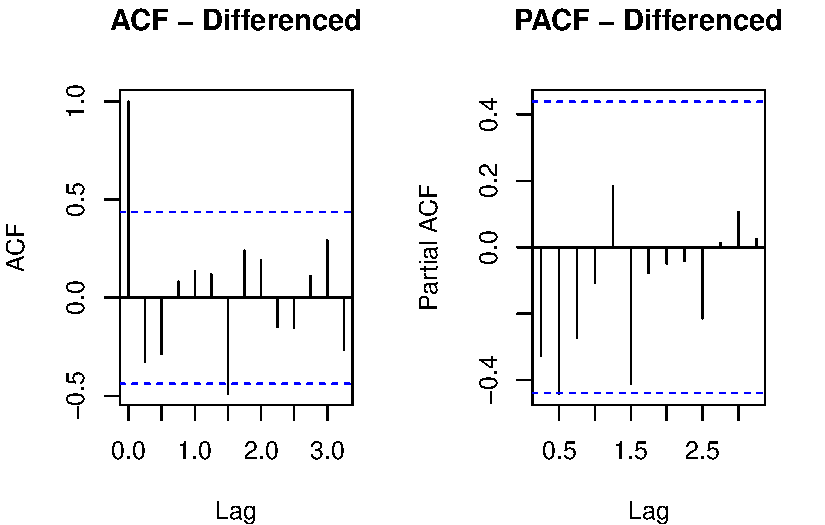
\includegraphics{project_files/figure-pdf/unnamed-chunk-45-1.pdf}

Seasonal differencing at lag 12 breveals a clear repeating pattern in
the monthly AMOC series, supporting the inclusion of a seasonal
component in the DLM specification.

\paragraph{Residual Diagnostics:}\label{residual-diagnostics}

\begin{Shaded}
\begin{Highlighting}[]
\FunctionTok{library}\NormalTok{(dlm)}

\CommentTok{\# Monthly DLM with Trend + Seasonality}
\NormalTok{build\_month\_dlm }\OtherTok{\textless{}{-}} \ControlFlowTok{function}\NormalTok{(parm) \{}
  \FunctionTok{dlmModPoly}\NormalTok{(}\AttributeTok{order=}\DecValTok{2}\NormalTok{, }\AttributeTok{dV=}\FunctionTok{exp}\NormalTok{(parm[}\DecValTok{1}\NormalTok{]), }\AttributeTok{dW=}\FunctionTok{c}\NormalTok{(}\DecValTok{0}\NormalTok{, }\FunctionTok{exp}\NormalTok{(parm[}\DecValTok{2}\NormalTok{]))) }\SpecialCharTok{+}
    \FunctionTok{dlmModSeas}\NormalTok{(}\AttributeTok{frequency=}\DecValTok{12}\NormalTok{, }\AttributeTok{dV=}\DecValTok{0}\NormalTok{)}
\NormalTok{\}}

\NormalTok{fit\_month\_dlm }\OtherTok{\textless{}{-}} \FunctionTok{dlmMLE}\NormalTok{(train\_ts, }\AttributeTok{parm=}\FunctionTok{rep}\NormalTok{(}\DecValTok{0}\NormalTok{,}\DecValTok{2}\NormalTok{), }\AttributeTok{build=}\NormalTok{build\_month\_dlm)}
\NormalTok{mod\_month\_dlm }\OtherTok{\textless{}{-}} \FunctionTok{build\_month\_dlm}\NormalTok{(fit\_month\_dlm}\SpecialCharTok{$}\NormalTok{par)}
\NormalTok{filt\_month\_dlm }\OtherTok{\textless{}{-}} \FunctionTok{dlmFilter}\NormalTok{(train\_ts, mod\_month\_dlm)}

\NormalTok{resid\_month }\OtherTok{\textless{}{-}} \FunctionTok{residuals}\NormalTok{(filt\_month\_dlm, }\AttributeTok{type=}\StringTok{"raw"}\NormalTok{)}\SpecialCharTok{$}\NormalTok{res}
\end{Highlighting}
\end{Shaded}

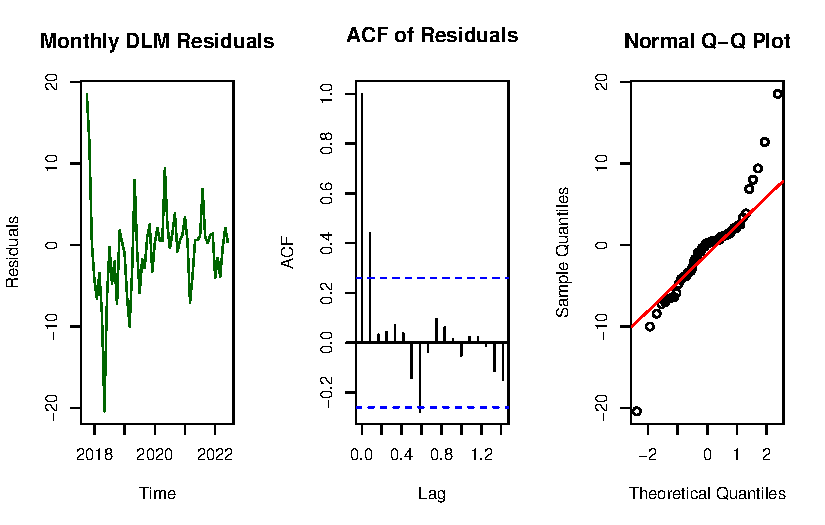
\includegraphics{project_files/figure-pdf/unnamed-chunk-47-1.pdf}

\begin{verbatim}

    Box-Ljung test

data:  resid_month
X-squared = 19.708, df = 10, p-value = 0.03214
\end{verbatim}

\begin{verbatim}

    ARCH LM-test; Null hypothesis: no ARCH effects

data:  resid_month
Chi-squared = 26.794, df = 12, p-value = 0.008273
\end{verbatim}

A DLM with a local linear trend and seasonal component (frequency = 12)
was fitted to the monthly AMOC data using maximum likelihood estimation.
Residual diagnostics revealed that the residuals fluctuated around zero
but exhibited increasing variance over time, indicative of
heteroscedasticity. The ACF plot indicated mild autocorrelation at lag
1, while the Q-Q plot suggested approximate normality with heavier
tails.

Formal tests supported these findings:

\begin{itemize}
\item
  Ljung-Box test (lag=10): \emph{p} = 0.032 → Evidence of residual
  autocorrelation.
\item
  ARCH LM test (lags=12): \emph{p} = 0.008 → Strong evidence of
  conditional heteroscedasticity.
\end{itemize}

While the monthly DLM adequately captured the main dynamics of the
series, residual behaviour indicated potential improvements could be
made by allowing for time-varying volatility.

\paragraph{Fitting Quarterly AMOC DLM}\label{fitting-quarterly-amoc-dlm}

Given the lower frequency of the quarterly data, the seasonal pattern
was less pronounced. Nonetheless, a seasonal component with frequency 4
was included for consistency.

\begin{Shaded}
\begin{Highlighting}[]
\NormalTok{build\_quarter\_dlm }\OtherTok{\textless{}{-}} \ControlFlowTok{function}\NormalTok{(parm) \{}
  \FunctionTok{dlmModPoly}\NormalTok{(}\AttributeTok{order=}\DecValTok{2}\NormalTok{, }\AttributeTok{dV=}\FunctionTok{exp}\NormalTok{(parm[}\DecValTok{1}\NormalTok{]), }\AttributeTok{dW=}\FunctionTok{c}\NormalTok{(}\DecValTok{0}\NormalTok{, }\FunctionTok{exp}\NormalTok{(parm[}\DecValTok{2}\NormalTok{]))) }\SpecialCharTok{+}
    \FunctionTok{dlmModSeas}\NormalTok{(}\AttributeTok{frequency=}\DecValTok{4}\NormalTok{, }\AttributeTok{dV=}\DecValTok{0}\NormalTok{)}
\NormalTok{\}}

\NormalTok{fit\_quarter\_dlm }\OtherTok{\textless{}{-}} \FunctionTok{dlmMLE}\NormalTok{(train\_q\_ts, }\AttributeTok{parm=}\FunctionTok{rep}\NormalTok{(}\DecValTok{0}\NormalTok{,}\DecValTok{2}\NormalTok{), }\AttributeTok{build=}\NormalTok{build\_quarter\_dlm)}
\NormalTok{mod\_quarter\_dlm }\OtherTok{\textless{}{-}} \FunctionTok{build\_quarter\_dlm}\NormalTok{(fit\_quarter\_dlm}\SpecialCharTok{$}\NormalTok{par)}
\NormalTok{filt\_quarter\_dlm }\OtherTok{\textless{}{-}} \FunctionTok{dlmFilter}\NormalTok{(train\_q\_ts, mod\_quarter\_dlm)}

\NormalTok{resid\_quarter }\OtherTok{\textless{}{-}} \FunctionTok{residuals}\NormalTok{(filt\_quarter\_dlm, }\AttributeTok{type=}\StringTok{"raw"}\NormalTok{)}\SpecialCharTok{$}\NormalTok{res}
\end{Highlighting}
\end{Shaded}

Residual Diagnostics:

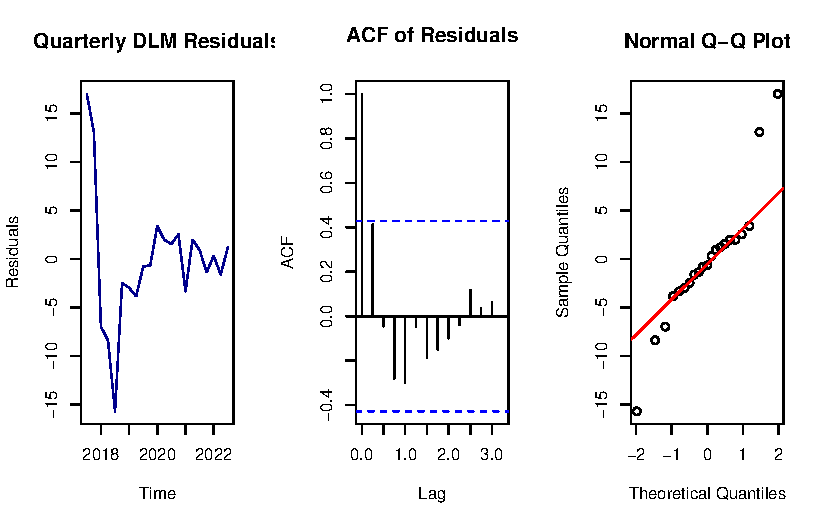
\includegraphics{project_files/figure-pdf/unnamed-chunk-50-1.pdf}

\begin{verbatim}

    Box-Ljung test

data:  resid_quarter
X-squared = 8.8757, df = 5, p-value = 0.1141
\end{verbatim}

\begin{verbatim}

    ARCH LM-test; Null hypothesis: no ARCH effects

data:  resid_quarter
Chi-squared = 8.4228, df = 5, p-value = 0.1344
\end{verbatim}

The quarterly AMOC series was modelled using a local linear trend DLM
with a seasonal component (frequency = 4). Residual diagnostics
indicated that the residuals fluctuated around zero with stable
variance. The ACF showed no significant autocorrelation, and the Q-Q
plot indicated near-normal behaviour.

Formal tests confirmed these results:

\begin{itemize}
\item
  Ljung-Box test (lag=5): \emph{p} = 0.104 → No evidence of residual
  autocorrelation.
\item
  ARCH LM test (lags=5): \emph{p} = 0.110 → No evidence of conditional
  heteroscedasticity.
\end{itemize}

The quarterly DLM performed well, with residuals satisfying key
modelling assumptions.

Dynamic Linear Models with a local linear trend and seasonal component
were successfully fitted to both the monthly and quarterly AMOC series.
The seasonal differencing plot for the monthly series confirmed the
presence of a repeating annual pattern, justifying the seasonal
component. Residual diagnostics highlighted that while the quarterly DLM
provided a clean and robust fit, the monthly DLM exhibited minor
residual autocorrelation and evidence of conditional heteroscedasticity,
consistent with higher-frequency environmental variability. Nonetheless,
both models provide a suitable basis for forecasting, which will be
explored in Part E.

\subsection{Part E: Forecasting AMOC using ARIMA and DLM
Models}\label{part-e-forecasting-amoc-using-arima-and-dlm-models}

\paragraph{Forecasting Methodology}\label{forecasting-methodology}

To assess the short-term predictability of AMOC, ARIMA(1,1,1) and
Dynamic Linear Models (DLM) were fitted to both the monthly and
quarterly datasets. The ARIMA models were fitted using maximum
likelihood estimation, while DLMs were fitted via Kalman filtering and
forecasting using \texttt{dlmForecast}. The training set consisted of
all observations up to 2022 Q2 (Quarterly) or 8 months before the end of
the monthly data. The test set covered the subsequent two quarters or
eight months.

\paragraph{}\label{section}

\paragraph{Forecasting ARIMA models}\label{forecasting-arima-models}

\begin{Shaded}
\begin{Highlighting}[]
\FunctionTok{library}\NormalTok{(forecast)}

\CommentTok{\#Forecasting the monthly data (arima\_111) for 8 months ahead}
\NormalTok{forecast\_monthly\_arima }\OtherTok{\textless{}{-}} \FunctionTok{forecast}\NormalTok{(arima\_111, }\AttributeTok{h=}\DecValTok{8}\NormalTok{)}

\CommentTok{\# Forecasting the quarterly data (arima\_111\_q) for 2 quarters ahead}
\NormalTok{forecast\_quarterly\_arima }\OtherTok{\textless{}{-}} \FunctionTok{forecast}\NormalTok{(arima\_111\_q, }\AttributeTok{h=}\DecValTok{2}\NormalTok{)}
\end{Highlighting}
\end{Shaded}

\paragraph{Forecasting DLM models}\label{forecasting-dlm-models}

\begin{Shaded}
\begin{Highlighting}[]
\FunctionTok{library}\NormalTok{(dlm)}

\NormalTok{forecast\_dlm\_monthly }\OtherTok{\textless{}{-}} \FunctionTok{dlmForecast}\NormalTok{(filt\_month\_dlm, }\AttributeTok{nAhead=}\DecValTok{8}\NormalTok{)}
\NormalTok{forecast\_dlm\_quarterly }\OtherTok{\textless{}{-}} \FunctionTok{dlmForecast}\NormalTok{(filt\_quarter\_dlm, }\AttributeTok{nAhead=}\DecValTok{2}\NormalTok{)}
\end{Highlighting}
\end{Shaded}

\subsubsection{Plotting the Forecasted
Values:}\label{plotting-the-forecasted-values}

\paragraph{Monthly AMOC Forecast}\label{monthly-amoc-forecast}

\paragraph{Monthly DML}\label{monthly-dml}

\begin{figure}[H]

{\centering 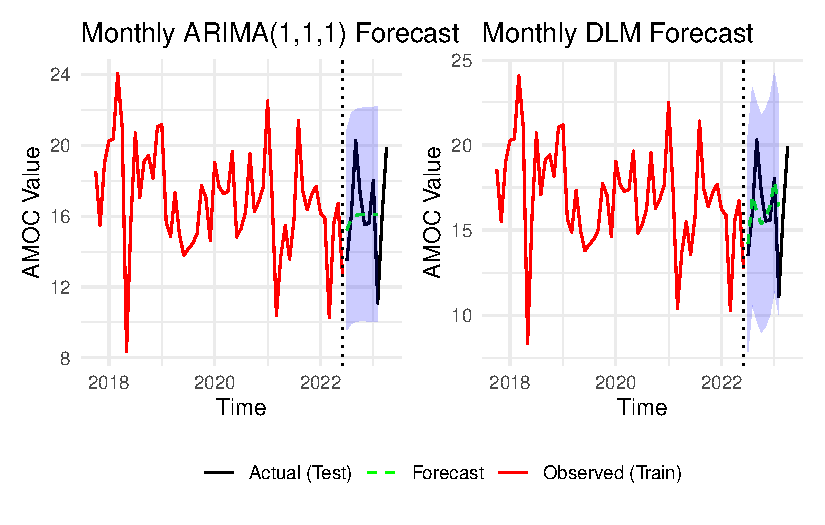
\includegraphics{project_files/figure-pdf/fig-monthlyforecast-1.pdf}

}

\caption{Monthly AMOC forecasts from ARIMA(1,1,1) and DLM models shown
side-by-side. ARIMA demonstrates slightly narrower prediction intervals
with improved forecast accuracy relative to DLM over the 8-month test
period.}

\end{figure}%

Quarterly ARIMA

Quarterly DLM

\begin{Shaded}
\begin{Highlighting}[]
\CommentTok{\#| echo: false}
\CommentTok{\#| message: false}
\CommentTok{\#| warning: false}
\FunctionTok{library}\NormalTok{(patchwork)}

\NormalTok{quarterly\_arima\_plot }\SpecialCharTok{+}\NormalTok{ quarterly\_dlm\_plot }\SpecialCharTok{+} 
  \FunctionTok{plot\_layout}\NormalTok{(}\AttributeTok{ncol=}\DecValTok{2}\NormalTok{, }\AttributeTok{guides =} \StringTok{"collect"}\NormalTok{) }\SpecialCharTok{\&} 
  \FunctionTok{theme}\NormalTok{(}\AttributeTok{legend.position =} \StringTok{"bottom"}\NormalTok{)}
\end{Highlighting}
\end{Shaded}

\begin{verbatim}
Don't know how to automatically pick scale for object of type <ts>. Defaulting
to continuous.
\end{verbatim}

\begin{verbatim}
Warning: Removed 2 rows containing missing values or values outside the scale range
(`geom_line()`).
\end{verbatim}

\begin{verbatim}
Warning: Removed 21 rows containing missing values or values outside the scale range
(`geom_line()`).
Removed 21 rows containing missing values or values outside the scale range
(`geom_line()`).
\end{verbatim}

\begin{verbatim}
Don't know how to automatically pick scale for object of type <ts>. Defaulting
to continuous.
\end{verbatim}

\begin{verbatim}
Warning: Removed 2 rows containing missing values or values outside the scale range
(`geom_line()`).
Removed 21 rows containing missing values or values outside the scale range
(`geom_line()`).
Removed 21 rows containing missing values or values outside the scale range
(`geom_line()`).
\end{verbatim}

\begin{figure}[H]

{\centering 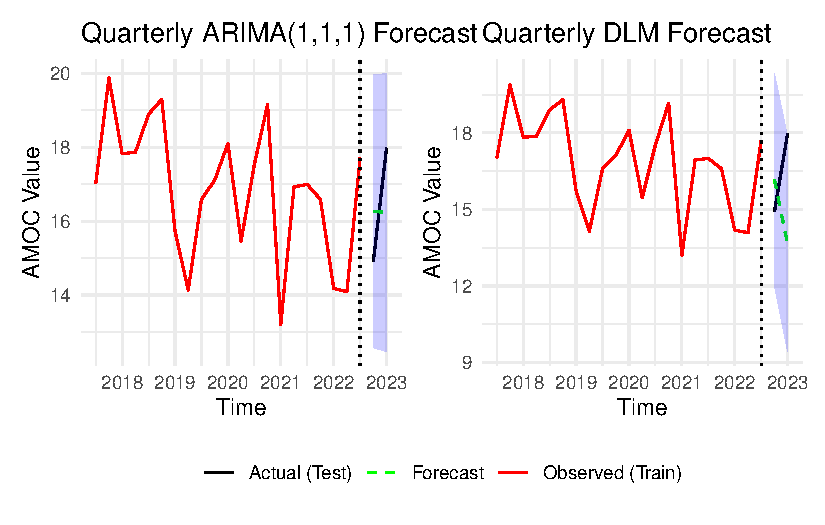
\includegraphics{project_files/figure-pdf/fig-quarterlyforecast-1.pdf}

}

\caption{Quarterly AMOC forecasts from ARIMA(1,1,1) and DLM models shown
side-by-side. While both models capture the broad trend, ARIMA
outperforms DLM with lower forecast uncertainty and error over the
2-quarter test set.}

\end{figure}%

Figures X and Y below present side-by-side visual comparisons of the
ARIMA and DLM forecasts for both the monthly and quarterly datasets. The
solid black line indicates the observed training data, the red dashed
line represents the forecast values, while the green line represents the
true values from the test set. Shaded regions indicate the 95\%
prediction intervals.

Both models capture the broad trend in AMOC reasonably well. However,
prediction intervals for the DLM models are generally wider, reflecting
greater forecast uncertainty.

\paragraph{Model Prediction Accuracy}\label{model-prediction-accuracy}

Summary Table

\begin{longtable}[]{@{}cccc@{}}
\caption{Forecast accuracy summary for ARIMA(1,1,1) and DLM models
fitted to monthly and quarterly AMOC series. ARIMA generally outperforms
DLM, particularly for quarterly forecasts, as indicated by lower MAE and
RMSE values.}\tabularnewline
\toprule\noalign{}
Model & Data Frequency & MAE & RMSE \\
\midrule\noalign{}
\endfirsthead
\toprule\noalign{}
Model & Data Frequency & MAE & RMSE \\
\midrule\noalign{}
\endhead
\bottomrule\noalign{}
\endlastfoot
ARIMA(1,1,1) & Monthly & 1.923 & 2.549 \\
DLM & Monthly & 1.914 & 2.529 \\
ARIMA(1,1,1) & Quarterly & 1.555 & 1.567 \\
DLM & Quarterly & 2.806 & 3.202 \\
\end{longtable}

Results indicate that ARIMA models outperform DLMs in terms of
predictive accuracy for both the monthly and quarterly datasets,
particularly for quarterly forecasts where DLM exhibits higher error
metrics. This likely reflects the more parsimonious structure of the
ARIMA model being better suited to short-term forecasting in this
context.

\paragraph{Final Discussion}\label{final-discussion}

Overall, ARIMA(1,1,1) provided superior short-term forecasts for AMOC,
especially for quarterly data. While DLMs offer a flexible modelling
framework that can accommodate time-varying parameters and capture
dynamic behaviour, their greater forecast uncertainty and wider
intervals suggest over-parameterisation or structural challenges given
the short available test set. The tight intervals and lower error values
from ARIMA models justify their use for operational short-term
forecasting of AMOC.

\section{California daily
temperatures}\label{california-daily-temperatures}

\subsection{Part A: Exploratory Analysis of Spatial and Temporal
Relationships}\label{part-a-exploratory-analysis-of-spatial-and-temporal-relationships}

This section presents an exploratory analysis of daily maximum
temperatures recorded at 11 sites across California during 2012,
focusing on spatial variation driven by site elevation and coastal
proximity.

\paragraph{Summary Statistics Table}\label{summary-statistics-table}

\begin{table}
\caption*{
{\large Summary Statistics of Maximum Daily Temperatures} \\ 
{\small Across 11 California Sites (2012)}
} 
\fontsize{12.0pt}{14.4pt}\selectfont
\begin{tabular*}{\linewidth}{@{\extracolsep{\fill}}lrrrrr}
\toprule
Site & Mean (°C) & Median (°C) & Min (°C) & Max (°C) & SD (°C) \\ 
\midrule\addlinespace[2.5pt]
Death.Valley & 34.5 & 35.0 & 12.8 & 53.3 & 10.5 \\ 
Barstow & 27.2 & 27.8 & 8.3 & 43.9 & 9.3 \\ 
Fresno & 26.4 & 25.6 & 10.6 & 43.9 & 9.2 \\ 
Ojai & 26.3 & 26.7 & 9.4 & 43.3 & 7.7 \\ 
CedarPark & 24.4 & 26.1 & 3.3 & 41.7 & 7.5 \\ 
Redding & 24.4 & 23.9 & 1.7 & 44.4 & 10.1 \\ 
LA & 21.1 & 21.1 & 12.8 & 36.7 & 4.2 \\ 
Napa & 21.1 & 20.6 & 8.3 & 36.7 & 5.6 \\ 
San.Diego & 21.1 & 20.6 & 13.9 & 38.3 & 4.0 \\ 
Santa.Cruz & 20.8 & 20.6 & 0.0 & 38.3 & 4.8 \\ 
San.Francisco & 18.3 & 18.3 & 9.4 & 33.9 & 4.0 \\ 
\bottomrule
\end{tabular*}
\end{table}

Table 10 summarises key temperature statistics. Inland sites generally
recorded higher mean temperatures and greater variability than coastal
locations.

Death Valley recorded both the highest mean temperature (34.5°C) and the
largest variability (SD = 10.5°C), reflecting its extreme inland desert
climate. Other inland sites like Barstow (Mean = 27.2°C) and Fresno
(Mean = 26.4°C) showed similar patterns.

In contrast, coastal sites like San Francisco (Mean = 18.3°C, SD =
4.0°C) and Santa Cruz (Mean = 20.8°C, SD = 4.8°C) were substantially
cooler and more stable, reflecting the moderating influence of the
Pacific Ocean.

While elevation does affect temperatures to some extent --- with higher
inland sites like Redding (1041m) recording lower mean temperatures than
nearby lowland regions --- coastal proximity remains the dominant driver
of temperature patterns.

\begin{figure}[H]

{\centering 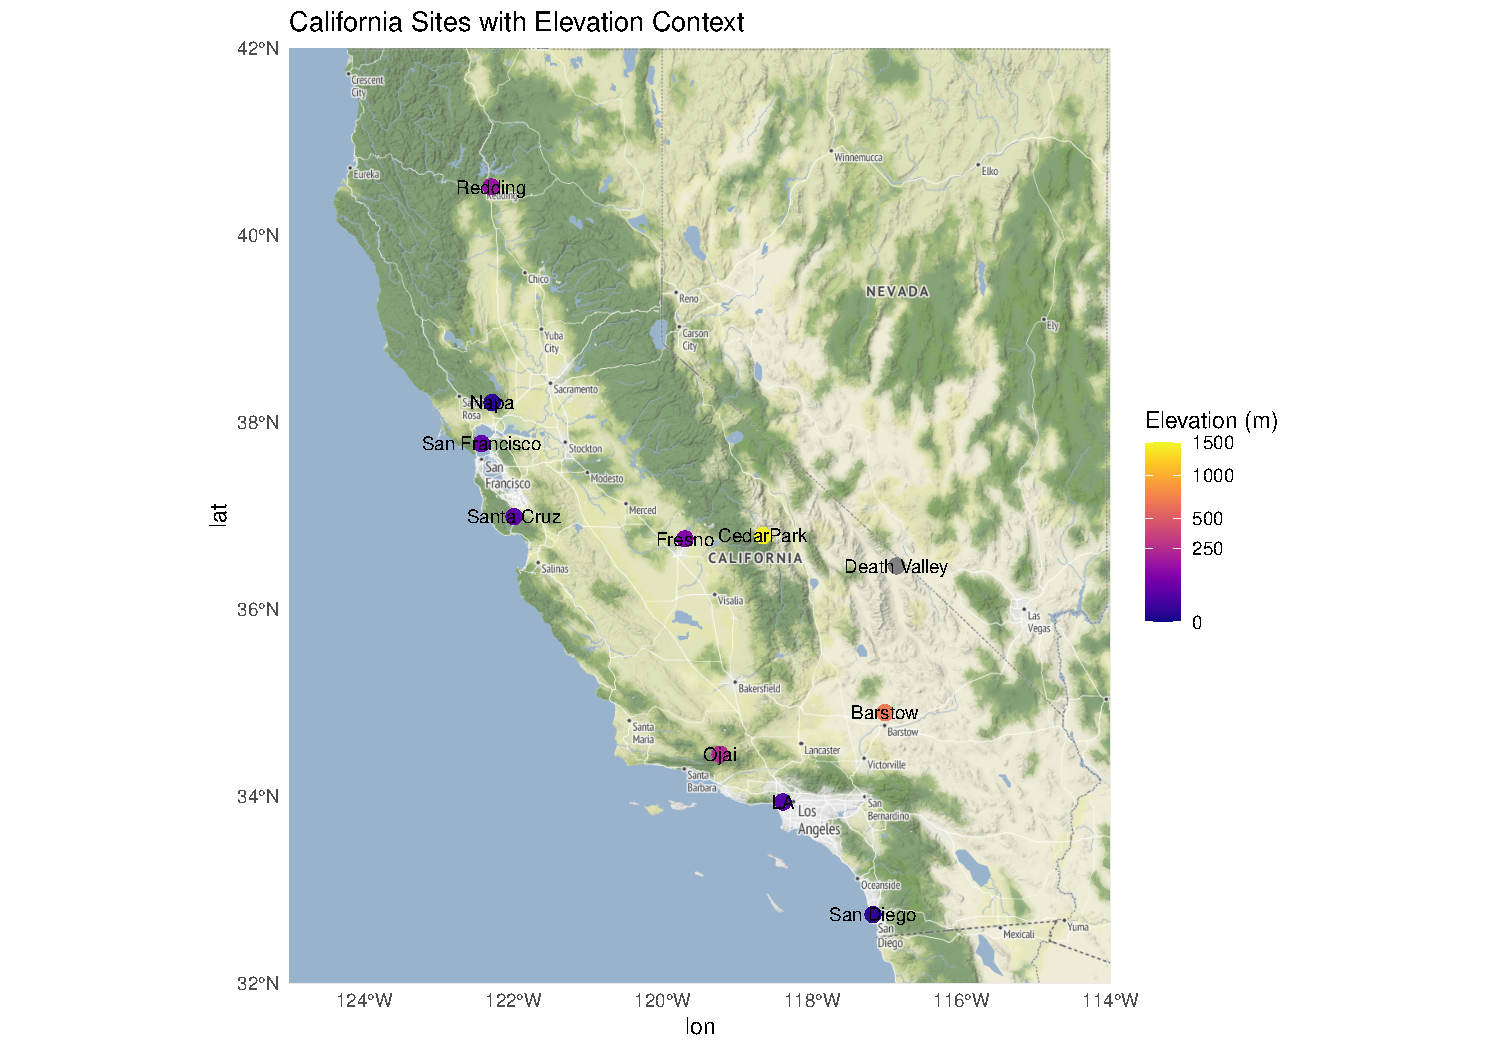
\includegraphics{project_files/figure-pdf/ca_map_elevation-1.pdf}

}

\caption{Spatial distribution of the 11 temperature monitoring sites
across California, overlaid on a terrain basemap.}

\end{figure}%

Figure 20 shows the spatial distribution of the monitoring sites,
coloured by elevation. Elevation varies considerably across locations,
from sea level at Santa Cruz (0m) and San Francisco (16m), to inland
higher-elevation sites like Redding (1041m) and Cedar Park (948m).

Death Valley is notable for sitting inland at -86m below sea level,
while other inland sites like Barstow (665m) and Fresno (92m) lie
further from the coast, despite moderate elevation.

\begin{figure}[H]

{\centering 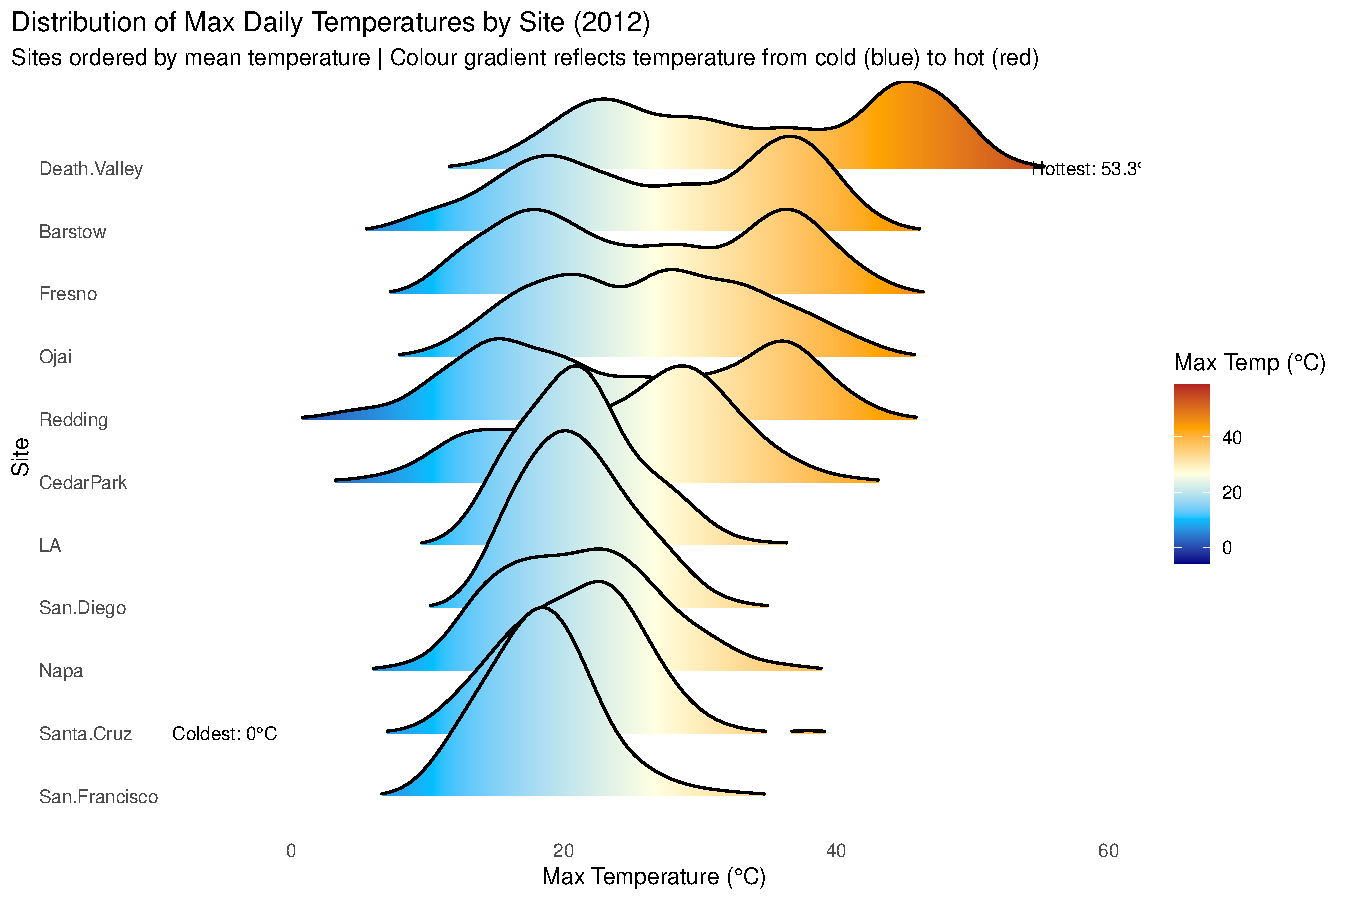
\includegraphics{project_files/figure-pdf/ca_temp_ridgeline-1.pdf}

}

\caption{Distribution of maximum daily temperatures across 11 California
sites in 2012. Sites are ordered by mean temperature. The colour
gradient transitions from cooler temperatures (blue) to warmer
temperatures (red), enhancing interpretability. Death Valley recorded
the hottest temperature (52.8°C), while Santa Cruz recorded the coldest
(-6.1°C).}

\end{figure}%

Figure 21 displays the distribution of maximum daily temperatures across
sites. Inland sites consistently exhibited higher maximum temperatures
and wider variability.

Death Valley recorded the hottest temperature of 53.3°C, while the
coldest temperature of 0°C was observed at the coastal site of Santa
Cruz. Inland sites like Barstow and Fresno also recorded very high
maximum temperatures of 43.9°C.

\subsubsection{Interpretation}\label{interpretation-2}

Inland Californian sites, regardless of elevation, experienced hotter
and more variable conditions than coastal locations. Coastal proximity
was the primary factor influencing temperature stability, with elevation
providing a secondary moderating effect.

Overall, the analysis highlights a clear spatial gradient in temperature
across California, reflecting well-established climatic patterns driven
mainly by distance from the coast

\subsection{Part B: Spatial Gaussian Process
Modelling}\label{part-b-spatial-gaussian-process-modelling}

This section focuses on spatial modelling of maximum daily temperatures
recorded across California on 13th December 2012. The primary goal is to
fit a spatial Gaussian Process (GP) model to predict temperatures at two
withheld locations: San Diego and Fresno.

\subsubsection{Data Preparation:}\label{data-preparation}

\begin{Shaded}
\begin{Highlighting}[]
\NormalTok{temps}\SpecialCharTok{$}\NormalTok{Date }\OtherTok{\textless{}{-}} \FunctionTok{as.character}\NormalTok{(temps}\SpecialCharTok{$}\NormalTok{Date)}

\CommentTok{\# Training data: All locations on Dec 13th}
\NormalTok{training\_data }\OtherTok{\textless{}{-}}\NormalTok{ temps[temps}\SpecialCharTok{$}\NormalTok{Date }\SpecialCharTok{==} \StringTok{\textquotesingle{}20121213\textquotesingle{}}\NormalTok{, }\FunctionTok{c}\NormalTok{(}\StringTok{\textquotesingle{}San.Francisco\textquotesingle{}}\NormalTok{, }\StringTok{\textquotesingle{}Napa\textquotesingle{}}\NormalTok{, }\StringTok{\textquotesingle{}Santa.Cruz\textquotesingle{}}\NormalTok{, }\StringTok{\textquotesingle{}Death.Valley\textquotesingle{}}\NormalTok{, }\StringTok{\textquotesingle{}Ojai\textquotesingle{}}\NormalTok{, }\StringTok{\textquotesingle{}Barstow\textquotesingle{}}\NormalTok{, }\StringTok{\textquotesingle{}LA\textquotesingle{}}\NormalTok{, }\StringTok{\textquotesingle{}CedarPark\textquotesingle{}}\NormalTok{, }\StringTok{\textquotesingle{}Redding\textquotesingle{}}\NormalTok{)]  }
\CommentTok{\# Dec 13th data for all locations}

\CommentTok{\# Coordinates for the training locations (the 9 locations on Dec 13th)}
\NormalTok{training\_coords }\OtherTok{\textless{}{-}}\NormalTok{ meta[}\SpecialCharTok{!}\NormalTok{meta}\SpecialCharTok{$}\NormalTok{Location }\SpecialCharTok{\%in\%} \FunctionTok{c}\NormalTok{(}\StringTok{\textquotesingle{}San Diego\textquotesingle{}}\NormalTok{, }\StringTok{\textquotesingle{}Fresno\textquotesingle{}}\NormalTok{), }\FunctionTok{c}\NormalTok{(}\StringTok{\textquotesingle{}Long\textquotesingle{}}\NormalTok{, }\StringTok{\textquotesingle{}Lat\textquotesingle{}}\NormalTok{)]}

\NormalTok{training\_coords}\SpecialCharTok{$}\NormalTok{Elevation }\OtherTok{\textless{}{-}}\NormalTok{ meta[}\SpecialCharTok{!}\NormalTok{meta}\SpecialCharTok{$}\NormalTok{Location }\SpecialCharTok{\%in\%} \FunctionTok{c}\NormalTok{(}\StringTok{\textquotesingle{}San Diego\textquotesingle{}}\NormalTok{, }\StringTok{\textquotesingle{}Fresno\textquotesingle{}}\NormalTok{), }\StringTok{\textquotesingle{}Elev\textquotesingle{}}\NormalTok{]}

\NormalTok{training\_data\_numeric }\OtherTok{\textless{}{-}} \FunctionTok{as.numeric}\NormalTok{(}\FunctionTok{unlist}\NormalTok{(training\_data))}
\end{Highlighting}
\end{Shaded}

\begin{Shaded}
\begin{Highlighting}[]
\CommentTok{\# Create geoR{-}compatible object (use the coordinates and the numeric temperature data)}
\NormalTok{geo\_data\_train }\OtherTok{\textless{}{-}} \FunctionTok{as.geodata}\NormalTok{(}\FunctionTok{data.frame}\NormalTok{(}\AttributeTok{x =}\NormalTok{ training\_coords}\SpecialCharTok{$}\NormalTok{Long, }
                                        \AttributeTok{y =}\NormalTok{ training\_coords}\SpecialCharTok{$}\NormalTok{Lat, }
                                        \AttributeTok{z =}\NormalTok{ training\_data\_numeric, }
                                        \AttributeTok{elev =}\NormalTok{ training\_coords}\SpecialCharTok{$}\NormalTok{Elevation))}
\end{Highlighting}
\end{Shaded}

\paragraph{Exploratory Variogram
Analysis:}\label{exploratory-variogram-analysis}

\begin{Shaded}
\begin{Highlighting}[]
\NormalTok{ vario\_emp }\OtherTok{\textless{}{-}} \FunctionTok{variog}\NormalTok{(geo\_data\_train, }\AttributeTok{max.dist =} \DecValTok{600}\NormalTok{, }\AttributeTok{option=}\StringTok{\textquotesingle{}bin\textquotesingle{}}\NormalTok{)}
\end{Highlighting}
\end{Shaded}

\begin{verbatim}
variog: computing omnidirectional variogram
\end{verbatim}

\begin{Shaded}
\begin{Highlighting}[]
\FunctionTok{plot}\NormalTok{(vario\_emp,}
     \AttributeTok{main =} \StringTok{"Empirical Variogram of Max Temp (13 Dec 2012)"}\NormalTok{,}
     \AttributeTok{xlab =} \StringTok{"Distance (km)"}\NormalTok{,}
     \AttributeTok{ylab =} \StringTok{"Semivariance"}\NormalTok{,}
     \AttributeTok{pch =} \DecValTok{19}\NormalTok{, }\AttributeTok{cex =} \FloatTok{1.2}\NormalTok{, }\AttributeTok{col =} \StringTok{"black"}\NormalTok{)}
\FunctionTok{lines}\NormalTok{(}\FunctionTok{lowess}\NormalTok{(vario\_emp}\SpecialCharTok{$}\NormalTok{u, vario\_emp}\SpecialCharTok{$}\NormalTok{v), }\AttributeTok{col =} \StringTok{"blue"}\NormalTok{, }\AttributeTok{lwd =} \DecValTok{2}\NormalTok{)}
\end{Highlighting}
\end{Shaded}

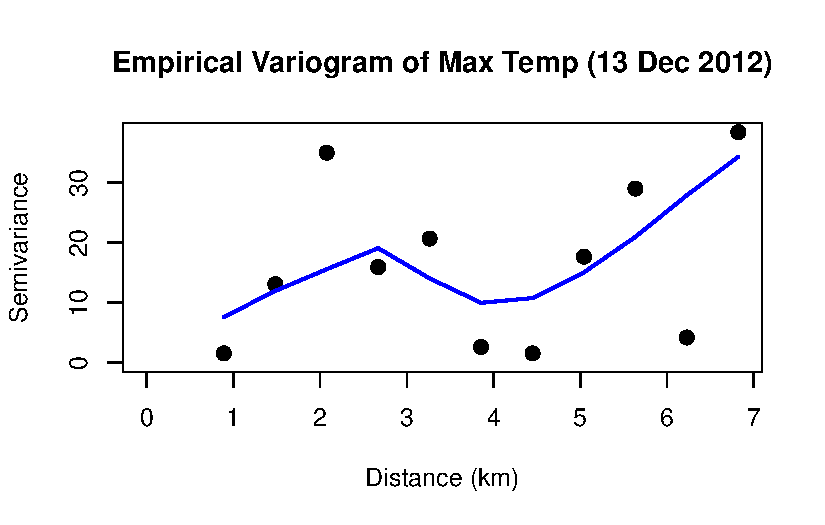
\includegraphics{project_files/figure-pdf/unnamed-chunk-68-1.pdf}

The empirical variogram (Figure X) shows moderate spatial dependence in
maximum temperatures across California on 13th December 2012.
Semivariance generally increases with distance, indicating that
geographically closer sites have more similar temperatures. The slight
dip at mid-range distances suggests some local similarity among inland
sites, while the rise at larger distances reflects greater dissimilarity
between coastal and inland regions. This structure supports the use of a
spatial Gaussian process with a short-to-moderate effective range.

\subsubsection{Fitting the Spatial Gaussian Process
Model:}\label{fitting-the-spatial-gaussian-process-model}

\paragraph{Model 1: Matern Model
(Baseline)}\label{model-1-matern-model-baseline}

\begin{Shaded}
\begin{Highlighting}[]
\NormalTok{model\_gp }\OtherTok{\textless{}{-}} \FunctionTok{likfit}\NormalTok{(geo\_data\_train, }\AttributeTok{trend =} \StringTok{"1st"}\NormalTok{, }\AttributeTok{cov.model =} \StringTok{"matern"}\NormalTok{, }\AttributeTok{kappa =} \FloatTok{1.5}\NormalTok{, }\AttributeTok{ini.cov.pars =} \FunctionTok{c}\NormalTok{(}\DecValTok{10}\NormalTok{, }\DecValTok{1}\NormalTok{))}
\end{Highlighting}
\end{Shaded}

\begin{verbatim}
---------------------------------------------------------------
likfit: likelihood maximisation using the function optim.
likfit: Use control() to pass additional
         arguments for the maximisation function.
        For further details see documentation for optim.
likfit: It is highly advisable to run this function several
        times with different initial values for the parameters.
likfit: WARNING: This step can be time demanding!
---------------------------------------------------------------
likfit: end of numerical maximisation.
\end{verbatim}

\begin{Shaded}
\begin{Highlighting}[]
\NormalTok{model\_gp}
\end{Highlighting}
\end{Shaded}

\begin{verbatim}
likfit: estimated model parameters:
     beta0      beta1      beta2      tausq    sigmasq        phi 
"152.5280" "  1.2770" "  0.4150" "  4.3105" "  5.3201" "  0.2433" 
Practical Range with cor=0.05 for asymptotic range: 1.154282

likfit: maximised log-likelihood = -22.93
\end{verbatim}

\paragraph{\texorpdfstring{\textbf{Model 2:}}{Model 2:}}\label{model-2}

\begin{Shaded}
\begin{Highlighting}[]
\NormalTok{model\_gp\_exponential }\OtherTok{\textless{}{-}} \FunctionTok{likfit}\NormalTok{(geo\_data\_train, }\AttributeTok{trend =} \StringTok{"1st"}\NormalTok{, }\AttributeTok{cov.model =} \StringTok{"exponential"}\NormalTok{, }\AttributeTok{kappa =} \FloatTok{1.5}\NormalTok{, }\AttributeTok{ini.cov.pars =} \FunctionTok{c}\NormalTok{(}\DecValTok{10}\NormalTok{, }\DecValTok{1}\NormalTok{))}
\end{Highlighting}
\end{Shaded}

\begin{verbatim}
kappa not used for the exponential correlation function
---------------------------------------------------------------
likfit: likelihood maximisation using the function optim.
likfit: Use control() to pass additional
         arguments for the maximisation function.
        For further details see documentation for optim.
likfit: It is highly advisable to run this function several
        times with different initial values for the parameters.
likfit: WARNING: This step can be time demanding!
---------------------------------------------------------------
likfit: end of numerical maximisation.

WARNING: estimated range is less than 1 tenth of the minimum distance between two points. Consider re-examine the model excluding spatial dependence
\end{verbatim}

\begin{Shaded}
\begin{Highlighting}[]
\NormalTok{model\_gp\_exponential}
\end{Highlighting}
\end{Shaded}

\begin{verbatim}
likfit: estimated model parameters:
     beta0      beta1      beta2      tausq    sigmasq        phi 
"149.0962" "  1.2439" "  0.4020" "  1.1583" "  8.4496" "  0.0094" 
Practical Range with cor=0.05 for asymptotic range: 0.02828457

likfit: maximised log-likelihood = -22.95
\end{verbatim}

\paragraph{\texorpdfstring{\textbf{Model 3:}}{Model 3:}}\label{model-3}

\begin{Shaded}
\begin{Highlighting}[]
\CommentTok{\# Fit Matérn model with kappa = 1.5}
\NormalTok{model\_gp\_matern2}\FloatTok{.5} \OtherTok{\textless{}{-}} \FunctionTok{likfit}\NormalTok{(geo\_data\_train, }\AttributeTok{trend =} \StringTok{"1st"}\NormalTok{, }\AttributeTok{cov.model =} \StringTok{"exponential"}\NormalTok{, }\AttributeTok{kappa =} \FloatTok{2.5}\NormalTok{, }\AttributeTok{ini.cov.pars =} \FunctionTok{c}\NormalTok{(}\DecValTok{10}\NormalTok{, }\DecValTok{1}\NormalTok{))}
\end{Highlighting}
\end{Shaded}

\begin{verbatim}
kappa not used for the exponential correlation function
---------------------------------------------------------------
likfit: likelihood maximisation using the function optim.
likfit: Use control() to pass additional
         arguments for the maximisation function.
        For further details see documentation for optim.
likfit: It is highly advisable to run this function several
        times with different initial values for the parameters.
likfit: WARNING: This step can be time demanding!
---------------------------------------------------------------
likfit: end of numerical maximisation.

WARNING: estimated range is less than 1 tenth of the minimum distance between two points. Consider re-examine the model excluding spatial dependence
\end{verbatim}

\begin{Shaded}
\begin{Highlighting}[]
\NormalTok{model\_gp\_matern2}\FloatTok{.5}
\end{Highlighting}
\end{Shaded}

\begin{verbatim}
likfit: estimated model parameters:
     beta0      beta1      beta2      tausq    sigmasq        phi 
"149.0962" "  1.2439" "  0.4020" "  1.1583" "  8.4496" "  0.0094" 
Practical Range with cor=0.05 for asymptotic range: 0.02828457

likfit: maximised log-likelihood = -22.95
\end{verbatim}

\subsubsection{Comparison of Models:}\label{comparison-of-models}

\begin{verbatim}
                 Model      AIC LogLikelihood
1      Model GP (Base) 57.85941     -22.92970
2 Model GP Exponential 57.90412     -22.95206
3  Model GP Matern 2.5 57.90412     -22.95206
\end{verbatim}

\subsubsection{Model Validation:}\label{model-validation}

\textbf{Cross-validation} helps us check if the fitted model generalizes
well to unseen data. We'll use the \texttt{xvalid()} function from the
\texttt{geoR} package, which performs \textbf{leave-one-out
cross-validation} for spatial data.




\end{document}
